%% ============================================================================
%% paper.tex
%% "The WKB Geometry of Newton Polygons: A Functorial Classification Theory"
%% Version: v1.0  (camera-ready candidate for Zenodo upload v1.0)
%% Companion dataset: doi:10.5281/zenodo.XXXXXXX  (PLACEHOLDER)
%% ============================================================================

\documentclass[11pt,a4paper]{article}

%% --- Geometry & typography -------------------------------------------------
\usepackage[margin=1in]{geometry}
\usepackage[T1]{fontenc}
\usepackage[utf8]{inputenc}
\usepackage{lmodern}
\usepackage{microtype}

%% --- Math ------------------------------------------------------------------
\usepackage{amsmath, amssymb, amsthm, mathtools}
\usepackage{mathrsfs}
\usepackage{stmaryrd}

%% --- Tables, lists, graphics, color ---------------------------------------
\usepackage{booktabs}
\usepackage{array}
\usepackage{enumitem}
\usepackage{graphicx}
\usepackage{xcolor}

%% --- Hyperlinks & cross-refs (load late) ----------------------------------
\usepackage[colorlinks=true,
            linkcolor=blue!50!black,
            citecolor=blue!50!black,
            urlcolor=blue!50!black]{hyperref}
\usepackage[capitalize,noabbrev]{cleveref}

%% --- Theorem environments --------------------------------------------------
\theoremstyle{plain}
\newtheorem{theorem}{Theorem}[section]
\newtheorem{lemma}[theorem]{Lemma}
\newtheorem{proposition}[theorem]{Proposition}
\newtheorem{corollary}[theorem]{Corollary}

\theoremstyle{definition}
\newtheorem{definition}[theorem]{Definition}
\newtheorem{example}[theorem]{Example}
\newtheorem{construction}[theorem]{Construction}

\theoremstyle{remark}
\newtheorem{remark}[theorem]{Remark}
\newtheorem{notation}[theorem]{Notation}

%% --- Macros (notation lock) -----------------------------------------------
\newcommand{\op}{\mathop{\square}}                % abstract irregular operator
\newcommand{\opD}{\mathrm{D}}                     % d/dx
\newcommand{\opS}{\mathrm{S}}                     % shift
\newcommand{\opT}{\mathrm{T}}                     % q-shift
\newcommand{\LCinf}{\mathrm{LC}_\infty}
\newcommand{\Roots}{\mathrm{Roots}}
\newcommand{\NL}{N(L)}
\newcommand{\NLa}{N(L)}
\newcommand{\Cl}{\mathcal{C}}
\newcommand{\Fclass}{\mathsf{F}}
\newcommand{\MW}{\mathrm{MW}}
\newcommand{\Sys}{\mathrm{Sys}}
\newcommand{\Sym}{\mathrm{Sym}}
\newcommand{\Symm}{\mathfrak{S}}
\newcommand{\disc}{\mathrm{disc}}
\newcommand{\Aset}{\mathcal{A}}
\newcommand{\Acov}{\mathcal{A}^{\mathrm{cov}}}
\newcommand{\Abase}{\mathcal{A}^{\mathrm{base}}}
\newcommand{\Dij}{\Delta_{ij}}
\newcommand{\ie}{i.e.\ }
\newcommand{\eg}{e.g.\ }
\newcommand{\cf}{cf.\ }
\newcommand{\Zlc}{\mathbb{Z}[\zeta_q]}
\newcommand{\Qlc}{\mathbb{Q}(\zeta_q)}
\newcommand{\sloped}[2]{-#1/#2}
\DeclareMathOperator{\arginline}{arg}
\newcommand{\Argm}{\arginline}

%% --- Title & authors -------------------------------------------------------
\title{The WKB Geometry of Newton Polygons:\\
       A Functorial Classification Theory}

\author{%
  Papanokechi\thanks{Independent researcher. ORCID:
  \href{https://orcid.org/0009-0000-6192-8273}{\texttt{0009-0000-6192-8273}}.
  Code and data repository:
  \url{https://github.com/papanokechi}.}
}

\date{\today\hspace{1ex}\textsc{(preprint v1.0)}}


\begin{document}
\maketitle

%% ============================================================================
%% ABSTRACT
%% ============================================================================
\begin{abstract}
For a scalar local linear operator $L$ (differential, difference, or
$q$-difference) with one irregular singularity at $x = \infty$ whose
Newton polygon has a unique dominant edge of slope $-p/q$ with $r{+}1$
lattice points, the WKB ansatz on that edge produces a characteristic
polynomial $\chi \in \mathbb{C}[c]$. Our central algebraic identity is
\[
   \chi(c) \;=\; \chi_w(c^q),
\]
where $\chi_w \in \mathbb{C}[w]$ is the classical edge-indicial polynomial
of degree $r$ in $w = c^q$. The exponent constellation
$\Cl(L) \subset \mathbb{C}$ is therefore a $\mu_q$-equivariant union of
$r$ fibres of $c \mapsto c^q$ over $\Roots(\chi_w)$.

This factorisation organises a finite stratified atlas: a computational
sweep yields $23$ single-edge classes for
$-p/q \in \{1/2,\,1/3,\,1/4,\,2/3,\,3/2\}$ and $r \le 3$, refining to
$39$ once multi-edge, nested-ramification, and prime-$q$ arithmetic
strata are tracked. We prove a per-edge factorisation along the slope
filtration, an iterated $\mu_{q'}$-pullback law for nested inner
polynomials, a block-diagonal pullback for systems, and a prime-$q$
Kummer dichotomy separating the algebraically independent stratum from
the cyclotomic stratum.

The analytic input attaching anti-Stokes directions is classical
(Levelt--Turrittin, Sibuya, Wasow); on the $q$-fold cover the rays of a
generic single-edge operator satisfy
$\arg \Dij + p\phi \equiv \pi/2 \pmod{\pi}$. One explicit consequence:
the slope numerator $p$, invisible to $\Cl(L)$, is visible to the
cover-side ray pattern. The analytic statements
(Theorems~\ref{thm:AT1}, \ref{thm:AT3}, \ref{thm:AT5}, \ref{thm:AT7})
are $\mu_q/\mu_{q'}$-equivariant repackagings of classical
formal-classification theory.
\end{abstract}

\bigskip
\noindent\textsc{Keywords:} WKB analysis; Newton polygon; irregular
singularity; formal classification; Levelt--Turrittin; Stokes phenomenon;
anti-Stokes directions; wild character variety; functorial classification;
$\mu_q$-pullback.

\bigskip
\noindent\textsc{MSC2020:} 34M40 (primary); 34M30, 34M35, 39A06, 39A13
(secondary).

\tableofcontents

\bigskip\hrule\bigskip


%% ============================================================================
%% §1  INTRODUCTION
%% ============================================================================
\section{Introduction}\label{sec:intro}

\subsection{The constellation map}\label{ssec:intro-functor}

To a scalar linear operator $L$ with a single irregular singularity at
$x = \infty$, the WKB ansatz on the dominant Newton edge attaches a
finite multiset of complex numbers, the \emph{exponent constellation}
\[
   \Cl(L) \;\subset\; \mathbb{C}.
\]
The present paper is about the combinatorial geometry of the
assignment
\[
   \Fclass \colon L \;\longmapsto\; \Cl(L),
\]
which we call the \emph{constellation map}. An earlier draft of this
paper used the word ``functor'' for $\Fclass$ informally; this revision
reserves that word for the precise categorical setting given in
\Cref{def:F-functor} below and otherwise speaks of the
\emph{constellation map}. In the body of the paper $\Fclass$ is treated
as a map between sets of objects (scalar local models with one dominant
Newton edge on the source side, finite multisets in $\mathbb{C}$ up to
global rotation on the target). \Cref{def:F-functor} promotes this to
a functor between two small categories whose morphisms are formal gauge
equivalences preserving the designated edge (source) and rotation-
compatible bijections of multisets (target); no statement in the paper
depends on the morphism part of $\Fclass$, but the formulation pins
down what we mean by ``the fibres of $\Fclass$''.

\begin{definition}[The category $\mathfrak{L}$ and the constellation
functor]\label{def:F-functor}
Let $\mathfrak{L}$ be the category whose
\begin{itemize}[leftmargin=2em]
\item \emph{objects} are pairs $(L, \mathfrak{e})$, where $L$ is a
scalar linear operator on $\mathbb{C}[x]$ in $\{\opD, \opS, \opT\}$
with exactly one irregular singularity at $x = \infty$ and
$\mathfrak{e}$ is a designated dominant edge of $\NL$ at infinity;
\item \emph{morphisms} $(L, \mathfrak{e}) \to (L', \mathfrak{e}')$
are formal gauge equivalences $\widehat{M}(L) \xrightarrow{\sim}
\widehat{M}(L')$ over $\mathbb{C}((x^{-1}))$ that send
$\mathfrak{e}$ to $\mathfrak{e}'$ under the induced action on Newton
polygons.
\end{itemize}
Let $\mathfrak{C}$ be the category whose
\begin{itemize}[leftmargin=2em]
\item \emph{objects} are finite multisets $C \subset \mathbb{C}$
taken up to the global rotation equivalence
$C \sim e^{i\theta} C$ for $\theta \in \mathbb{R}/2\pi\mathbb{Z}$;
\item \emph{morphisms} are multiset bijections compatible with the
rotation action.
\end{itemize}
The assignment $(L, \mathfrak{e}) \mapsto \Cl(L)$, extended to morphisms
by sending a formal gauge equivalence to the induced bijection of
roots of $\chi$, defines a functor
\[
   \Fclass \colon \mathfrak{L} \;\longrightarrow\; \mathfrak{C}.
\]
\end{definition}

\begin{remark}\label{rem:F-functoriality}
Functoriality is immediate from the construction of $\chi$ from the
leading-coefficient data along $\mathfrak{e}$: a formal gauge
equivalence preserving $\mathfrak{e}$ acts on the $\LCinf$-data of
$\mathfrak{e}$ by a cocycle that preserves $\chi$ up to an overall
rescaling of $c$, and hence preserves the multiset of roots of $\chi$
up to a global rotation. We will use ``$\Fclass$'' and ``the
constellation map'' interchangeably in the remainder of the paper.
Whenever only the underlying object map matters, the reader may
forget \Cref{def:F-functor} without loss.
\end{remark}

\subsection{The structural law}\label{ssec:intro-law}

The central observation, proved in \Cref{thm:main}, is the algebraic
identity
\[
   \chi(c) \;=\; \chi_w(c^q),
\]
where $\chi$ is the WKB characteristic polynomial built from the
$\LCinf$-data along the dominant edge and $\chi_w \in \mathbb{C}[w]$
is the \emph{inner polynomial} of degree $r$. Solving $\chi = 0$
amounts to solving $\chi_w$ in the variable $w = c^q$ and pulling
back along $c \mapsto c^q$; the constellation decomposes canonically
as a $\mu_q$-equivariant union of $r$ fibres over $\Roots(\chi_w)$.
This factorisation is at once an obstruction (no multiset outside the
image of $\Fclass$ admits it) and a recipe (every multiset in the
image is so built). \Cref{sec:main} states the law as
\Cref{thm:main} with two corollaries (ring decomposition; Vieta
monodromy) and a remark on the degeneracy strata.

\subsection{$\chi_w$ as the edge-indicial polynomial}
\label{ssec:intro-chi-w}

The polynomial $\chi_w$ is not new content. It is exactly the
\emph{edge-indicial polynomial} of the dominant edge $\mathfrak{e}$
in the variable $w = c^q$, the form that appears in the classical
leading-balance analysis of irregular singularities (Wasow
\cite{wasow}, Sibuya \cite{sibuya}, Sabbah
\cite{sabbah-isomon}). Setting $w = c^q$, the equation $\chi_w(w) = 0$
is the standard requirement that the WKB ansatz produce a
non-trivial formal solution along $\mathfrak{e}$. The novelty of
\Cref{thm:main} is therefore not the existence of $\chi_w$ but the
clean identification
\[
   \chi(c) \;=\; \chi_w(c^q),
\]
together with the consequence that the $\mu_q$-equivariant fibre
structure of $\Cl(L)$ becomes explicit, and the slope denominator $q$
appears as a \emph{pullback index} rather than as a feature of the
leading balance to be rediscovered case by case.

\subsection{From a law to a classification}
\label{ssec:intro-classification}

The structural law turns the classification problem into a
combinatorial one. Up to global rotation, a constellation is recovered
from $(p, q, r)$ together with the modulus-with-multiplicity partition
$\pi$ of the roots of $\chi_w$. A computational sweep, recorded in the
companion dataset \cite{wkb_dataset_v1}, enumerates these classes for
slopes $-p/q \in \{1/2, 1/3, 1/4, 2/3, 3/2\}$ and ranks $r \in
\{1, 2, 3\}$ across three equation types: there are exactly $23$
classes in the single-edge case. Once multi-edge polygons, nested
ramification, and the prime-$q$ arithmetic stratification are recorded,
the atlas refines to $39$ classes. These populate the open stratum
and four named degenerate strata (equal modulus; resonant multiplicity;
zero root; accidental symmetry); \Cref{sec:classes} catalogues them.

The classification is extended in several directions:
\begin{itemize}[leftmargin=*]
\item beyond the single edge: per-edge factorisation along the slope
      filtration (\Cref{thm:M1}, \Cref{sec:multiedge});
\item beyond a single $\mu_q$-orbit: nested ramification with iterated
      pullbacks (\Cref{thm:N1}, \Cref{sec:multiedge});
\item beyond squarefree $\chi_w$: degeneracy strata and a prime-$q$
      Kummer dichotomy (\Cref{thm:D2}, \Cref{sec:degeneracy});
\item beyond scalar operators: block-diagonal systems and a
      symmetric-power target (\Cref{thm:S1}, \Cref{sec:systems});
\item beyond the discrete invariant: an analytic refinement attaching
      anti-Stokes directions to the differences $\Dij = c_i - c_j$
      (\Cref{thm:AT1,thm:AT3,thm:AT5,thm:AT7}, \Cref{sec:analytic}).
\end{itemize}

\subsection{Scope of the analytic refinement}
\label{ssec:intro-analytic-scope}

The analytic theorems of \Cref{sec:analytic} attach Stokes-side
information to the constellation. The reader should bear in mind a
clear division of labour:
\begin{itemize}[leftmargin=2em]
\item \emph{Classical content.} The Levelt--Turrittin slope
decomposition of a formal connection on a ramified cover of index $q$;
the existence of formal exponential factors $Q_i(t) = c_i t^p +
(\text{lower})$; the principle that anti-Stokes rays are governed by
the leading term of $Q_i - Q_j$; and the slope-graded structure of
Stokes data for multi-edge connections are classical
(Sibuya \cite{sibuya}, Wasow \cite{wasow}, Sabbah
\cite{sabbah-polarizable}).
\item \emph{Algebraic refinement.} What is new in the present paper
is the explicit linear form for the anti-Stokes condition in
\Cref{thm:AT1},
\[
   \arg \Dij \;+\; p\phi \;\equiv\; \tfrac{\pi}{2} \pmod \pi;
\]
the observation that nested factorisations of $\chi_w$ induce an
additional $\mu_{q'}$-action on the discrete part of the wild data
\emph{without} changing the ramification index $q$ (\Cref{thm:AT3});
the consequent $\mu_q/\mu_{q'}$ symmetry bookkeeping; and the
$p$-visibility statement \Cref{thm:AT7}, by which the slope numerator
$p$---invisible to $\Cl(L)$---is visible to the cover-side ray pattern.
\item \emph{Equivariance, not Stokes matrices.} \Cref{thm:AT3} asserts
$\mu_{q'}$-equivariance of an irregular-type parametrisation; it is
not a statement about wild character variety strata in the moduli-
theoretic sense of Boalch \cite{boalch-stokes,boalch-wildhodge}.
We are explicit about this distinction.
\end{itemize}

\subsection{What is and is not classified}\label{ssec:intro-scope}

The object classified in this paper is the image of $\Fclass$ over
the single-edge ($23$-class) and the extended single-edge / multi-edge
/ nested-ramification / system / arithmetic strata ($39$-class). We
do \emph{not} classify operators. The constellation is a coarsening of
the irregular-type data of Levelt--Turrittin, and the kernel of this
coarsening---operators with identical constellation but distinct
Stokes structures---is the complementary problem solved (in
appropriate categories) by wild character varieties (Boalch
\cite{boalch-stokes,boalch-wildhodge}). \Cref{sec:related} positions
the present work alongside neighbouring programmes: ADE
classifications of singularities; Stokes-graph and spectral-network
classifications; the formal classification of irregular connections
(Levelt--Turrittin, Sabbah \cite{sabbah-isomon,sabbah-polarizable},
Mochizuki \cite{mochizuki-asymptotic}); and wild character varieties.
The constellation classification is orthogonal to each.

\subsection{Roadmap}\label{ssec:intro-organisation}

\Cref{sec:prelim} fixes notation, recalls Newton polygons and the WKB
symbol, and includes a short notation table.
\Cref{sec:main} proves the structural law (\Cref{thm:main}).
\Cref{sec:multiedge} extends to multi-edge polygons via the slope-
filtration per-edge factorisation (\Cref{thm:M1}) and to nested
ramification (\Cref{thm:N1}).
\Cref{sec:degeneracy} treats the four degeneracy strata and proves the
prime-$q$ Kummer dichotomy (\Cref{thm:D2}), separating the algebraic
statement (Kummer theory over $\mathbb{Q}(\zeta_q)$) from the
empirical bounded-search corroboration.
\Cref{sec:systems} treats systems (\Cref{thm:S1}).
\Cref{sec:analytic} states and proves the four analytic-lifting
theorems (\Cref{thm:AT1,thm:AT3,thm:AT5,thm:AT7}), with explicit
hypotheses (OS1)--(OS5) collected in \Cref{ssec:OS}.
\Cref{sec:classes} presents the $23$-class atlas, the $39$-class
refinement, the taxonomy diagram (\Cref{fig:taxonomy}), and the
constellation zoo (\Cref{fig:zoo}).
\Cref{sec:related} positions the work alongside its neighbours,
\Cref{sec:vision} closes with future directions, and
\Cref{sec:reproducibility} contains a reproducibility note.

\bigskip
The reader interested only in the structural law may read
\Cref{sec:main} immediately after \Cref{sec:prelim}; the analytic
theorems of \Cref{sec:analytic} depend logically on
\Cref{sec:main,sec:multiedge} but may be read in any internal order.



%% ============================================================================
%% §2  PRELIMINARIES
%% ============================================================================
\section{Newton polygons and the WKB symbol}\label{sec:prelim}

\subsection{Operators and conventions}\label{ssec:prelim-ops}

We work over $\mathbb{C}$. Let $L$ be a scalar linear operator
\[
   L \;=\; \sum_{k=0}^{n}\, a_k(x)\, \op^{\,k},
   \qquad a_k \in \mathbb{C}[x],\ a_n \ne 0,
\]
where $\op$ is one of:
\begin{itemize}[leftmargin=2em]
\item $\opD := \mathrm{d}/\mathrm{d}x$ \quad (the \emph{ODE case}),
\item $\opS \colon f(x) \mapsto f(x+1)$ \quad (the \emph{difference case}),
\item $\opT \colon f(x) \mapsto f(qx)$ for fixed $|q| \ne 0, 1$ \quad
      (the \emph{$q$-difference case}; we reserve the symbol $q$ for the
      slope denominator below and use a separate parameter for the
      $q$-shift when both appear).
\end{itemize}
We assume $L$ has a single irregular singularity at $x = \infty$ and is
regular elsewhere. The coefficients $a_k$ are polynomial throughout; the
extension to formal Laurent series is straightforward and notationally
heavier without affecting the structural law.

\subsection{Newton polygon at infinity}\label{ssec:prelim-Newton}

For each $a_k \in \mathbb{C}[x] \setminus \{0\}$, write $\deg a_k$ for its
degree in $x$. The \emph{Newton polygon at infinity} of $L$ is
\[
   \NL \;:=\;
   \mathrm{ConvexHull}\big\{\,(k, \deg a_k) : a_k \ne 0\,\big\}
   \;-\; \mathrm{lower\ half\!-plane},
\]
\ie\ the upper convex hull of the support, viewed as a polygon in
$\mathbb{R}^2$. Edges of $\NL$ are line segments with slope $-p/q$ in
lowest terms ($\gcd(p, q) = 1$, $p, q \ge 1$), oriented so that the slope
decreases left-to-right.

\begin{definition}[Dominant edge]\label{def:dominant-edge}
A \emph{dominant edge} of $\NL$ is an edge of strictly maximal slope. We
say $L$ has \emph{one dominant edge} if $\NL$ admits a unique such edge.
Multi-edge polygons are treated in \S\ref{sec:multiedge}.
\end{definition}

\begin{remark}[Equation-type independence of $N(L)$]\label{rem:Newton-uniform}
The Newton polygon is defined uniformly across $\opD$, $\opS$, $\opT$:
the recipe ``plot $(k, \deg a_k)$ and take the upper convex hull'' produces
the same polygon. The \emph{analytic} interpretation of an edge differs
(slope $-p/q$ means $f \sim \exp(c\, x^{p/q})$ for $\opD$, but
$f \sim \prod (\text{shift factors})$ for $\opS$ or $\opT$); the
\emph{combinatorial} content is identical.
\end{remark}

\begin{lemma}[Lattice points on an edge]\label{lem:lattice-on-edge}
Let $E$ be an edge of $\NL$ of slope $-p/q$ with $\gcd(p, q) = 1$. Then
the lattice points of $E$ are exactly
\[
   E \cap \mathbb{Z}^2
   \;=\;
   \big\{(k_0 + jq,\ h_0 - jp) : 0 \le j \le r\big\},
\]
where $(k_0, h_0)$ is the lower-right endpoint of $E$ and $r \ge 1$ is the
\emph{rank multiplier}. Equivalently, $E$ contains $r + 1$ lattice points
and has horizontal extent $rq$.
\end{lemma}

\begin{proof}
A vector $(\Delta k, \Delta h)$ along $E$ satisfies
$\Delta h / \Delta k = -p/q$. The primitive integer vector in this
direction is $(q, -p)$, and $\gcd(q, p) = 1$ ensures these are the only
lattice points lying on $E$ between its two endpoints, parametrised by
$j = 0, 1, \dots, r$ where $r$ is the integer length of $E$ measured in
multiples of $(q, -p)$.
\end{proof}

\subsection{The WKB symbol and the characteristic polynomial}\label{ssec:prelim-WKB}

Fix a dominant edge $E$ of slope $-p/q$ with lattice points
$(k_0 + jq,\ h_0 - jp)$, $0 \le j \le r$, as above. For each such lattice
point, write
\[
   \alpha_j
   \;:=\;
   \LCinf\big(a_{k_0 + jq}\big)
   \;\in\; \mathbb{C},
\]
where $\LCinf$ extracts the leading coefficient in $x$ at $\infty$.
(The lattice point lies on $E$ iff $a_{k_0 + jq}$ has degree exactly
$h_0 - jp$ in $x$, so $\alpha_j$ is unambiguous.)

\begin{definition}[WKB characteristic polynomial]\label{def:chi}
The \emph{WKB characteristic polynomial} of $L$ along the dominant edge $E$
is
\[
   \chi(c)
   \;:=\;
   \sum_{j=0}^{r}\, \alpha_j\, c^{(r-j)q}
   \;\in\; \mathbb{C}[c].
\]
The \emph{inner polynomial} is
\[
   \chi_w(w)
   \;:=\;
   \sum_{j=0}^{r}\, \alpha_j\, w^{\,r-j}
   \;\in\; \mathbb{C}[w],
   \qquad \deg \chi_w = r.
\]
The \emph{constellation} of $L$ is the multiset
$\Cl(L) := \Roots(\chi) \subset \mathbb{C}$, with roots counted with
multiplicity.
\end{definition}

\begin{remark}[Origin of $\chi$ from the WKB ansatz]\label{rem:chi-from-ansatz}
For $\op = \opD$, substituting $f = \exp\!\big(\frac{q}{p}\, c\, x^{p/q}\big)\,
g(x)$ into $L f = 0$ with $c$ to be determined gives, at leading order in
$x$, the equation $\sum_j \alpha_j\, c^{(r-j)q}\, x^{(r-j)p + h_0} = 0$ along
the edge $E$. Equating coefficients of the highest power of $x$ yields
$\chi(c) = 0$, recovering \Cref{def:chi}. For $\opS$, the substitution is
$f \sim \exp\!\big(\frac{c\, x^{1 + p/q}}{1 + p/q}\big)$ and the algebra is
identical; likewise for $\opT$ (with the appropriate logarithm). The
\emph{combinatorial} object $\chi$ is identical in all three cases; this
is the source of equation-type independence at the constellation level.
\end{remark}

\begin{notation}[The classification functor]\label{not:F}
For brevity we package $\Fclass \colon L \mapsto \Cl(L)$ as a map from the
category $\mathsf{Op}$ of scalar local irregular operators (up to formal
gauge fixing the leading edge) to the category $\mathsf{MSet}_\mathbb{C}$
of finite multisets in $\mathbb{C}$ modulo global rotation. ``Functor'' is
used here in the loose sense: the assignment respects formal gauge
equivalence; functoriality with respect to morphisms in $\mathsf{Op}$
(\eg\ pullback along a finite ramification, twist by an exponential)
is recorded as needed below.
\end{notation}

%% ---------------------------------------------------------------------------
%% Round-1 follow-up: consolidated notation table for the manuscript
%% ---------------------------------------------------------------------------
\begin{table}[t]
\centering
\small
\begin{tabular}{@{}ll@{}}
\toprule
\textbf{Symbol} & \textbf{Meaning} \\
\midrule
$L$            & scalar linear operator with one irregular singularity at $\infty$ \\
$\op \in \{\opD, \opS, \opT\}$
               & derivation, shift, or $q$-shift, respectively \\
$\NL$          & Newton polygon of $L$ at $\infty$ \\
$E$, $-p/q$, $r$
               & dominant edge; slope (lowest terms); rank multiplier \\
$\LCinf(\cdot)$ & leading coefficient at $x = \infty$ \\
$\chi(c)$, $\chi_w(w)$
               & WKB characteristic polynomial; inner polynomial ($\chi(c) = \chi_w(c^q)$) \\
$\Cl(L)$       & exponent constellation $= \Roots(\chi) \subset \mathbb{C}$ \\
$\Fclass$      & constellation map / functor $(L, \mathfrak{e}) \mapsto \Cl(L)$ \\
$\mu_q, \zeta_q$
               & group of $q$-th roots of unity; primitive root $e^{2\pi i / q}$ \\
$\Dij$         & pairwise difference $c_i - c_j$, $c_i, c_j \in \Cl(L)$ \\
$\Acov$        & anti-Stokes set on the $q$-fold cover $x = t^q$ \\
$\Zlc, \Qlc$   & cyclotomic ring $\mathbb{Z}[\zeta_q]$ and field $\mathbb{Q}(\zeta_q)$ \\
$R_\alpha$     & $\mu_q$-ring $\{\zeta_q^j z_\alpha : 0 \le j < q\}$ \\
\bottomrule
\end{tabular}
\caption{Notation used throughout the paper.}\label{tab:notation}
\end{table}


%% ============================================================================
%% §3  MAIN THEOREM
%% ============================================================================
\section{The Main Theorem}\label{sec:main}

We now state and prove the structural law that organises the rest of the
paper. Hypotheses are kept minimal: a scalar operator with one dominant
edge, in any of the three equation types.

\begin{theorem}[Factorisation of the WKB characteristic polynomial]\label{thm:main}
Let $L = \sum_{k=0}^{n} a_k(x)\, \op^{\,k}$ be a scalar linear operator with
polynomial coefficients $a_k \in \mathbb{C}[x]$ and a single irregular
singularity at $x = \infty$, where $\op \in \{\opD, \opS, \opT\}$. Assume
the Newton polygon $\NL$ at $\infty$ has a unique dominant edge $E$ of
slope $-p/q$ with $\gcd(p, q) = 1$ and $p, q \ge 1$, containing $r + 1$
lattice points
\[
   E \cap \mathbb{Z}^2 \;=\;
   \big\{(k_0 + jq,\ h_0 - jp) : 0 \le j \le r\big\}.
\]
Set $\alpha_j := \LCinf(a_{k_0 + jq})$ for $0 \le j \le r$, and define
$\chi(c)$ and $\chi_w(w)$ as in \Cref{def:chi}. Then
\[
   \boxed{\,
     \chi(c) \;=\; \chi_w(c^q),
   \,}
\]
and the WKB exponent constellation factors as the $\mu_q$-equivariant
fibre product
\[
   \Cl(L) \;=\; \Roots(\chi)
   \;=\;
   \bigsqcup_{w_i \in \Roots(\chi_w)}
   \big\{\, c \in \mathbb{C} : c^q = w_i \,\big\},
\]
where roots are counted with multiplicity and the union is over the $r$
roots $w_i$ of $\chi_w$.
\end{theorem}

\begin{proof}
By \Cref{def:chi},
$\chi(c) = \sum_{j=0}^{r} \alpha_j\, c^{(r-j) q}
       = \sum_{j=0}^{r} \alpha_j\, (c^q)^{r-j}
       = \chi_w(c^q).$
The factorisation of $\Cl(L)$ follows by substitution: $\chi(c) = 0$ iff
$c^q \in \Roots(\chi_w)$, and for each such $w_i$ the preimage under
$c \mapsto c^q$ is the $\mu_q$-orbit $\{c : c^q = w_i\}$. Multiplicities
in $\chi_w$ are transmitted to $\chi$ unchanged: if $w_i$ is a root of
$\chi_w$ of multiplicity $m_i$, then each $c$ with $c^q = w_i$ is a root
of $\chi$ of multiplicity $m_i$.
\end{proof}

\begin{corollary}[Generic ring decomposition]\label{cor:ring}
If the moduli $|w_1|, \dots, |w_r|$ are pairwise distinct and all
$w_i \ne 0$, then $\Cl(L)$ consists of exactly $r$ concentric
$\mu_q$-orbits (``rings'') of $q$ points each, with radii $|w_i|^{1/q}$
and angular bases $\arginline(w_i) / q \pmod{2\pi/q}$.
\end{corollary}

\begin{proof}
For each simple root $w_i$ of $\chi_w$, the fibre $\{c : c^q = w_i\}$
consists of $q$ points evenly spaced on the circle of radius
$|w_i|^{1/q}$, with one of them at angle $\arginline(w_i)/q$ and the others
obtained by multiplication by $\zeta_q^k$. The hypotheses make the
$r$ rings concentric and pairwise distinct.
\end{proof}

\begin{corollary}[Vieta monodromy]\label{cor:vieta}
Fix $\alpha_0$ and let $\beta := \alpha_r$ vary. Under $\beta \mapsto
e^{i\theta} \beta$,
\[
   \arginline\!\Big(\prod_{c \in \Cl(L)} c\Big)
   \;\longmapsto\;
   \arginline\!\Big(\prod_{c \in \Cl(L)} c\Big) \;+\; \theta \pmod{2\pi}.
\]
If $\Cl(L)$ admits a $\mu_q$-equivariant ring decomposition
$\Cl(L) = \bigsqcup_{k=1}^{s} R_k$ with $|R_k| = m_k$, and the rings deform
rigidly under the variation of $\beta$ with rotations $\Delta_k$ (each
defined modulo $2\pi / m_k$), then the unambiguous lifts $m_k \Delta_k \in
\mathbb{R}/2\pi\mathbb{Z}$ obey
\[
   \sum_{k=1}^{s} m_k\, \Delta_k \;\equiv\; \theta \pmod{2\pi}.
\]
\end{corollary}

\begin{proof}
Vieta's formula gives $\prod_{c \in \Roots(\chi)} c = (-1)^{\deg \chi}\,
\alpha_0 / \alpha_r$, so its argument is shifted by $-\theta$ under
$\alpha_r \mapsto e^{i\theta} \alpha_r$ (sign convention absorbed). For the
ring lift: each ring $R_k$ contributes $m_k \Delta_k$ to the change in
$\arginline \prod c$ (the per-ring rotations are well-defined modulo
$2\pi/m_k$, and the lift $m_k \Delta_k$ is unambiguous). Summing and
matching to the total shift $\theta$ gives the rule.
\end{proof}

\begin{remark}[Degenerate loci]\label{rem:degenerate}
The clean ring picture of \Cref{cor:ring} fails on three explicit
subvarieties of coefficient space $(\alpha_0, \dots, \alpha_r)$:
\begin{enumerate}[label=(\roman*)]
\item the \emph{discriminant locus} $\{\disc \chi_w = 0\}$, where roots of
      $\chi_w$ coalesce and ring multiplicities exceed $q$;
\item the \emph{equal-modulus locus} $\{|w_i| = |w_j|$ for some $i \ne j\}$,
      where distinct $\mu_q$-orbits merge into a single radius with
      non-uniform angular distribution;
\item the \emph{zero-root locus} $\{\alpha_r = 0\}$, where $c = 0$ enters
      the constellation with multiplicity $q$ and the dominant edge itself
      jumps.
\end{enumerate}
The first carries resonance / logarithmic Stokes data; the second is
responsible for the apparent regularity of the
equal-modulus stratum (e.g.\ a six-point constellation on one circle
that is \emph{not} a regular hexagon); the third is a wall-crossing of
the Newton
polygon itself. \S\ref{sec:degeneracy} treats them systematically.
\end{remark}

\begin{remark}[Equation-type invariance]\label{rem:eq-invariance}
The proof of \Cref{thm:main} uses only the combinatorial identity
$c^{(r-j)q} = (c^q)^{r-j}$, no analytic input. Consequently, the
factorisation holds identically across $\opD$, $\opS$, $\opT$. The analytic
\emph{meaning} of $c \in \Cl(L)$ differs (it is the leading-order WKB
exponent $c$ in $f \sim \exp(c\, x^{p/q}/(p/q))$ for $\opD$; for $\opS$ it
is $\log(S f / f)|_\infty$ to leading order; for $\opT$ it is
$\log_q(T f / f)|_\infty$); the multiset $\Cl(L)$ is invariant. This is
the precise sense in which $\Fclass$ is equation-type independent.
\end{remark}

\begin{remark}[Forward references]\label{rem:forward-main}
\Cref{thm:main} is the base case of the entire programme. It generalises
in three directions: to multi-edge polygons (\Cref{thm:M1}); to nested
factorisations of $\chi_w$ (\Cref{thm:N1}); to systems (\Cref{thm:S1}).
The complementary analytic refinement
(\Cref{thm:AT1,thm:AT3,thm:AT5,thm:AT7}) attaches anti-Stokes directions
to the differences $\Dij = c_i - c_j$ on the ramified cover $x = t^q$.
\end{remark}


%% ============================================================================
%% §4  MULTI-EDGE AND NESTED RAMIFICATION
%% ============================================================================
\section{Multi-edge polygons and nested ramification}\label{sec:multiedge}

\subsection{Per-edge factorisation along the slope filtration}\label{ssec:M1}

When $N(L)$ has several edges of distinct slopes, the Main Theorem applies
per edge and the constellations assemble multiplicatively via the
formal-classification (Levelt--Turrittin) slope decomposition.

\begin{lemma}[Multiplicativity of the WKB characteristic polynomial
across slope-disjoint formal direct sums]\label{lem:chi-multiplicative}
Let $L_A$ and $L_B$ be scalar linear operators on $\mathbb{C}[x]$ in
$\{\opD, \opS, \opT\}$, each with a single irregular singularity at
$x = \infty$. Suppose that the Newton polygon $N(L_A)$ at $\infty$
consists of edges $E_1^A, \dots, E_{m_A}^A$ of distinct slopes
$-p_i^A / q_i^A$ ($i = 1, \dots, m_A$, $\gcd(p_i^A, q_i^A) = 1$,
$p_i^A, q_i^A \ge 1$), and that $N(L_B)$ consists of a \emph{single}
edge of slope $-p_B / q_B$ with $\gcd(p_B, q_B) = 1$, $p_B, q_B \ge 1$.
Assume the slope-disjointness hypothesis
\begin{equation}\label{eq:slope-disjoint}
   \frac{p_B}{q_B} \;\notin\; \Big\{\frac{p_1^A}{q_1^A},\,
   \dots,\, \frac{p_{m_A}^A}{q_{m_A}^A}\Big\}.
\end{equation}
Let $\widehat{M}(L_A) \oplus \widehat{M}(L_B)$ denote the formal direct
sum of the associated $\mathbb{C}((x^{-1}))$-modules, and let $L_{AB}$
be any scalar operator on $\mathbb{C}[x]$ obtained from a cyclic vector
for the direct sum. Then
\[
   \chi_{L_{AB}}(c) \;=\; \chi_{L_A}(c)\, \chi_{L_B}(c),
\]
where $\chi_{L_A}, \chi_{L_B}$ denote the WKB characteristic polynomials
of $L_A, L_B$ (the product, in the case of $L_A$, of its per-edge
characteristic polynomials over $E_1^A, \dots, E_{m_A}^A$).
\end{lemma}

\begin{proof}
The Newton polygon of a formal direct sum of irregular connections
equals the upper convex hull of the union of the Newton polygons of the
summands (\cite[Ch.~III, \S 1]{sabbah-isomon}; or, for the classical
scalar case, \cite[Ch.~II]{robba-malgrange}). Under
\eqref{eq:slope-disjoint}, this upper hull consists of $m_A + 1$ edges,
exactly one for each slope in $\{p_i^A/q_i^A\}_{i=1}^{m_A} \cup
\{p_B/q_B\}$.

We analyse the $\LCinf$-data along each edge $E$ of $N(L_{AB})$. There
are two cases.

\smallskip
\textit{Case 1: $E$ has slope $-p_i^A/q_i^A$ for some
$i \in \{1, \dots, m_A\}$.}
On the lattice $E \cap \mathbb{Z}^2$, only the summand $\widehat M(L_A)$
contributes leading-order ($\LCinf$) terms at slope $p_i^A/q_i^A$;
the summand $\widehat M(L_B)$ has a single slope $p_B/q_B \ne p_i^A/q_i^A$
and therefore contributes only lower-order ($x^{-1}$-higher-valuation)
corrections to the $\LCinf$-data on $E$. Hence
\[
   \LCinf\!\big(a_k^{(AB)}\big)\big|_{E}
   \;=\;
   \LCinf\!\big(a_k^{(A)}\big)\big|_{E_i^A}
   \qquad \text{for } (k, h) \in E \cap \mathbb{Z}^2,
\]
which by \Cref{def:chi} gives the per-edge identity
$\chi^{(i,A)}_{L_{AB}}(c) = \chi^{(i)}_{L_A}(c)$.

\smallskip
\textit{Case 2: $E$ has slope $-p_B/q_B$.}
By the same argument with the roles of $L_A$ and $L_B$ exchanged, the
$\LCinf$-data on $E$ is contributed solely by the (single edge of)
$\widehat M(L_B)$. Hence
$\chi^{(B)}_{L_{AB}}(c) = \chi_{L_B}(c)$.

\smallskip
Multiplying over all edges of $N(L_{AB})$ and using that for a scalar
operator with multiple slope-distinct edges the total WKB characteristic
polynomial is the product of its per-edge characteristic polynomials,
\[
   \chi_{L_{AB}}(c)
   \;=\;
   \Big(\prod_{i=1}^{m_A} \chi^{(i,A)}_{L_{AB}}(c)\Big)\,
   \chi^{(B)}_{L_{AB}}(c)
   \;=\;
   \Big(\prod_{i=1}^{m_A} \chi^{(i)}_{L_A}(c)\Big)\,
   \chi_{L_B}(c)
   \;=\;
   \chi_{L_A}(c)\, \chi_{L_B}(c),
\]
as claimed.
\end{proof}

\begin{remark}[Iteration over arbitrarily many slope-disjoint summands]
\label{rem:chi-mult-iteration}
The single-slope restriction on $L_B$ is essential only in the
inductive step; \emph{either} operand may be multi-slope provided the
slope-disjointness hypothesis~\eqref{eq:slope-disjoint} (interpreted as
disjointness of slope sets) holds. In particular, an obvious induction
on the number of slopes establishes the multi-fold multiplicativity
statement
\[
   \chi_{L_1 \oplus \cdots \oplus L_m}(c)
   \;=\;
   \prod_{\alpha=1}^{m}\, \chi_{L_\alpha}(c),
\]
where each $L_\alpha$ is single-slope of slope $-p_\alpha/q_\alpha$ and
the slopes are pairwise distinct. This is exactly the form invoked in
the proof of \Cref{thm:M1} (Step 3): one applies the lemma to
$(\widehat M_1 \oplus \cdots \oplus \widehat M_{m-1}) \oplus \widehat
M_m$, with $L_A := L_1 \oplus \cdots \oplus L_{m-1}$ a multi-slope
operator (with slope set $\{p_1/q_1, \dots, p_{m-1}/q_{m-1}\}$) and
$L_B := L_m$ single-slope with slope $p_m/q_m$ distinct from those of
$L_A$. The slope-disjointness hypothesis is exactly the multi-slope
hypothesis $p_i/q_i \neq p_j/q_j$ for $i \ne j$ in the parent operator
$L$.
\end{remark}

\begin{theorem}[Per-edge factorisation; multi-edge generalisation]\label{thm:M1}
Let $L$ be a scalar linear operator with polynomial coefficients on
$\mathbb{C}[x]$ and a single irregular singularity at $x = \infty$. Suppose
$\NL$ has edges $E_1, \dots, E_m$ with pairwise distinct slopes
$-p_\alpha / q_\alpha$ ($\gcd(p_\alpha, q_\alpha) = 1$) and $r_\alpha + 1$
lattice points on $E_\alpha$. Let $k_0^{(\alpha)}$ be the height of $E_\alpha$
above the $c$-axis, and let $\chi_w^{(\alpha)} \in \mathbb{C}[w]$ be the
inner polynomial of degree $r_\alpha$ built from the $\LCinf$ data of
$E_\alpha$ (per \Cref{def:chi}). Then:
\begin{enumerate}[leftmargin=2em]
\item (Slope decomposition.) The formal differential module
      $\widehat{M}(L)$ associated to $L$ at $x = \infty$ admits a canonical
      direct-sum decomposition $\widehat{M}(L) \simeq \bigoplus_{\alpha=1}^{m}
      \widehat{M}_\alpha$ with $\widehat{M}_\alpha$ of pure slope
      $p_\alpha / q_\alpha$. Choosing cyclic vectors realises each
      $\widehat{M}_\alpha$ as the formal module of a scalar single-slope
      operator $L_\alpha$, and we write
      $\widehat{L} \simeq L_1 \oplus \cdots \oplus L_m$.
\item (Per-edge characteristic polynomial.) Each $L_\alpha$ satisfies
      \Cref{thm:main} with
      $\chi^{(\alpha)}(c) = c^{k_0^{(\alpha)}}\, \chi_w^{(\alpha)}(c^{q_\alpha})$.
\item (Total factorisation.) Setting $\chi(c) := \prod_{\alpha=1}^{m}
      \chi^{(\alpha)}(c)$, one has
      $\Cl(L) = \bigsqcup_{\alpha=1}^{m} \Cl_\alpha$ as multisets, with
      $\Cl_\alpha := \Roots(\chi^{(\alpha)})$.
\end{enumerate}
On the open subset $U_{\mathrm{disj}}$ of coefficient space where the
per-edge radial annuli $[\rho_\alpha^{\min}, \rho_\alpha^{\max}]$ with
$\rho_\alpha^{\bullet} = |w^\bullet|^{1/q_\alpha}$ are pairwise disjoint,
the union is a disjoint union of \emph{distinct} subsets of $\mathbb{C}$.
\end{theorem}

\begin{proof}[Proof of \Cref{thm:M1} (Per-edge factorisation; multi-edge
generalisation)]
We organise the argument in four steps.

\smallskip
\textit{Step 1 (Slope decomposition; Levelt--Turrittin).}
By the Levelt--Turrittin theorem (Sibuya \cite{sibuya};
Wasow \cite[Ch.~VII]{wasow}; Sabbah \cite[Ch.~II,
Thm.~II.2.4]{sabbah-isomon}), the formal $\mathbb{C}((x^{-1}))$-module
$\widehat{M}(L)$ associated to $L$ at $x = \infty$ admits a canonical
slope decomposition
\[
   \widehat{M}(L) \;=\; \bigoplus_{\alpha=1}^{m}\,
   \widehat{M}_\alpha,
\]
where $\widehat{M}_\alpha$ is pure of slope $p_\alpha/q_\alpha$ and
the multiset $\{p_\alpha/q_\alpha\}_{\alpha=1}^{m}$ is exactly the set
of slopes of the edges of $N(L)$. The decomposition is canonical
(unique up to gauge), and choosing a cyclic vector in each summand
$\widehat{M}_\alpha$ realises it as the formal module of a scalar
single-slope operator $L_\alpha$. The Newton polygon of $L_\alpha$
consists of a single edge of slope $-p_\alpha/q_\alpha$ with
$r_\alpha + 1$ lattice points, matching the corresponding edge
$E_\alpha$ of $N(L)$.

\smallskip
\textit{Step 2 (Per-edge Main Theorem).}
Each $L_\alpha$ has Newton polygon $N(L_\alpha)$ a single edge of
slope $-p_\alpha/q_\alpha$ with $r_\alpha + 1$ lattice points;
\Cref{thm:main} applies and gives the explicit factorisation
\[
   \chi_{L_\alpha}(c)
   \;=\;
   c^{k_0^{(\alpha)}}\, \chi_w^{(\alpha)}(c^{q_\alpha}),
\]
where $k_0^{(\alpha)}$ is the multiplicity of $c = 0$ in $\chi_{L_\alpha}$
contributed by lattice points strictly below $E_\alpha$ (the
``foot'' of the edge in the scalar operator $L$), and
$\chi_w^{(\alpha)} \in \mathbb{C}[w]$ is the inner polynomial of
degree $r_\alpha$ built from the $\LCinf$-data of $E_\alpha$ per
\Cref{def:chi}.

\smallskip
\textit{Step 3 (Multiplicativity across the slope filtration).}
Apply \Cref{lem:chi-multiplicative} inductively to the $m$-fold
formal direct sum
\[
   \widehat{M}(L) \;=\; \widehat{M}_1 \oplus \cdots \oplus \widehat{M}_m
\]
(equivalently, $\widehat{L} \simeq L_1 \oplus \cdots \oplus L_m$, in
the sense of Step~1). The $m = 2$ case is \Cref{lem:chi-multiplicative}
directly; the inductive step is the identity $\widehat{M}_1 \oplus
\cdots \oplus \widehat{M}_m = (\widehat{M}_1 \oplus \cdots \oplus
\widehat{M}_{m-1}) \oplus \widehat{M}_m$ together with the
single-slope hypothesis on $\widehat{M}_m$ (its single slope
$p_m/q_m$ is distinct from those of the first $m - 1$ summands by
hypothesis on $L$). Hence
\[
   \chi_L(c)
   \;=\;
   \prod_{\alpha=1}^{m}\, \chi_{L_\alpha}(c)
   \;=\;
   \prod_{\alpha=1}^{m}\,
   c^{k_0^{(\alpha)}}\, \chi_w^{(\alpha)}(c^{q_\alpha}).
\]
Taking roots with multiplicity,
\[
   \Cl(L) \;=\; \Roots(\chi_L)
   \;=\;
   \bigsqcup_{\alpha = 1}^{m}\, \Roots(\chi_{L_\alpha})
   \;=\;
   \bigsqcup_{\alpha = 1}^{m}\, \Cl_\alpha
\]
as multisets.

\smallskip
\textit{Step 4 (Genericity).}
On the open subset $U_{\mathrm{disj}}$ of coefficient space where
the per-edge radial annuli
\[
   \big[\rho_\alpha^{\min},\, \rho_\alpha^{\max}\big],
   \qquad
   \rho_\alpha^{\bullet}
   \;=\;
   \min_w / \max_w\!\big\{|w|^{1/q_\alpha} : w \in
   \Roots(\chi_w^{(\alpha)})\big\},
\]
are pairwise disjoint as subsets of $\mathbb{R}_{> 0}$, the multiset
union $\bigsqcup_\alpha \Cl_\alpha$ is also an honest disjoint union
of subsets of $\mathbb{C}^\times$, because the per-edge constellations
occupy disjoint moduli. On the complement (the radii-collision
stratum), the multiset disjoint union is preserved by Step~3; only
the set-theoretic statement in $\mathbb{C}^\times$ is weakened,
namely, distinct edges may contribute roots of equal absolute value.
\end{proof}

\begin{remark}\label{rem:M1-cyclic-vector}
The choice of cyclic vector in Step~1 affects the scalar operator
$L_\alpha$ only up to a formal gauge equivalence; this gauge preserves
$\chi_{L_\alpha}$ (\Cref{rem:F-functoriality}), so the per-edge
characteristic polynomials $\chi^{(\alpha)}$ depend canonically on
$\widehat{M}_\alpha$ and hence on the edge $E_\alpha$. The statement
of \Cref{thm:M1} is therefore intrinsic.
\end{remark}

\begin{remark}[Counterexample boundary for M1]\label{rem:M1-counter}
The disjoint-union conclusion in (3) is a multiset statement; as
\emph{sets} in $\mathbb{C}^\times$ the per-edge constellations may
coincide on the \emph{inter-edge equal-radius stratum}, where the
radial annuli of two distinct edges accidentally share a radius.
Examples are documented in the companion dataset \cite{wkb_dataset_v1}.
Likewise, when a per-edge $\chi_w^{(\alpha)}(0) = 0$, the zero-root
contributions of adjacent edges \emph{share} the origin in $\mathbb{C}$.
These are not contradictions: the multiset disjoint union is preserved;
only the set-theoretic statement is weakened.
\end{remark}

\subsection{Nested ramification}\label{ssec:N1}

Beyond a single $\mu_q$-pullback, the inner polynomial $\chi_w$ itself
may factor through a higher power.

\begin{theorem}[Nested ramification: iterated $\mu_q$-pullback]\label{thm:N1}
Let $L$ be scalar with one dominant edge of slope $-p/q$ as in
\Cref{thm:main}. Suppose the inner polynomial admits a factorisation
$\chi_w(w) = \chi_v(w^{q'})$ for some integer $q' \ge 2$ and a polynomial
$\chi_v \in \mathbb{C}[v]$ of degree $r' = r / q'$ (\ie\ $\chi_w$ has
nonzero coefficients only in degrees that are multiples of $q'$). Then
\[
   \Cl(L) \;=\; \bigsqcup_{v \in \Roots(\chi_v)}
            \big\{\, c \in \mathbb{C} : c^{qq'} = v \,\big\}.
\]
Each $v$-fibre $\{c : c^{qq'} = v\}$ has size $qq'$ and carries a free
$\mu_{qq'}$-action. The \emph{visible} symmetry group generated by the
outer $\mu_q$-action (from $\chi(c) = \chi_w(c^q)$) and the nested
$\mu_{q'}$-action (from $\chi_w = \chi_v \circ (\cdot)^{q'}$) is
\[
   \mu_{\mathrm{lcm}(q, q')} \;\subseteq\; \mu_{qq'},
\]
with equality $\mu_{\mathrm{lcm}(q, q')} = \mu_{qq'}$ if and only if
$\gcd(q, q') = 1$ (in which case $\mu_{qq'} \cong \mu_q \times \mu_{q'}$
canonically by CRT).
\end{theorem}

\begin{proof}
By \Cref{thm:main}, $\chi(c) = \chi_w(c^q)$; substituting the hypothesis
gives $\chi(c) = \chi_v\big((c^q)^{q'}\big) = \chi_v(c^{qq'})$. The fibre
decomposition follows. For the symmetry claim, the original Main
Theorem's $\mu_q$-action sits inside $\mu_{qq'}$ as the subgroup
$\{\zeta_{qq'}^{q' k}\}$. A lift to $c$-level of the inner-polynomial
$\mu_{q'}$-symmetry (acting on $w = c^q$ by $w \mapsto \zeta_{q'} w$) is
multiplication by an $\eta \in \mu_{qq'}$ with $\eta^q = \zeta_{q'}$;
such $\eta$ exists (\eg\ $\eta = \zeta_{qq'}^q$) and is unique modulo
$\mu_q$. The subgroup of $\mu_{qq'}$ generated by $\zeta_q$ and $\eta$
is $\mu_{\mathrm{lcm}(q, q')}$.
\end{proof}

\begin{remark}[Minimality]\label{rem:N1-min}
The hypothesis $\chi_w(w) = \chi_v(w^{q'})$ is preserved under further
inner factorisations $\chi_v(v) = \chi_u(v^{q''})$; iterating until no
inner factorisation is possible gives the \emph{minimal} $q' q'' \cdots$
through which the constellation factors. The companion atlas
\cite{wkb_dataset_v1} records two such nested operators, both stable
under one round of inner factorisation.
\end{remark}

\begin{remark}[Constellation vs.\ analytic ramification]\label{rem:N1-analytic}
\Cref{thm:N1} is a purely algebraic identity at the constellation level.
The analytic implications for the Levelt--Turrittin ramification cover are
deferred to \Cref{thm:AT3}; crucially, the minimal cover for the formal
classification remains $x = t^q$ and does not increase to $x = \tau^{qq'}$.
The nested factorisation refines the wild character variety, not the
ramification index.
\end{remark}


%% ============================================================================
%% §5  DEGENERACY STRATA AND ARITHMETIC STRATIFICATION
%% ============================================================================
\section{Degeneracy strata and arithmetic stratification}\label{sec:degeneracy}

The Main Theorem (\Cref{thm:main}) decomposes the image of $\Fclass$
into a generic stratum and the three degenerate loci of
\Cref{rem:degenerate}. We now treat the degeneracy strata and their
arithmetic refinement, culminating in a prime-$q$ Kummer dichotomy
(\Cref{thm:D2}).

\subsection{The four named strata}\label{ssec:strata-named}

In the companion atlas \cite{wkb_dataset_v1}, four stress-test operators
exhibit the qualitatively distinct degenerate behaviours:
\begin{enumerate}[leftmargin=2em]
\item \emph{Equal-modulus locus.} Six points on a single circle of
      radius $\sqrt{2}$, \emph{not} evenly spaced.
\item \emph{Discriminant locus} (resonant multiplicity): two rings, the
      inner with multiplicity $2$ at each apparent point.
\item \emph{Zero-root locus} (wall-crossing): two points at radius $1$
      together with a multiplicity-$q$ root at the origin.
\item \emph{Accidental-symmetry locus.} A regular $rq$-gon with cyclic
      symmetry $C_{rq} \supsetneq C_q$, occurring at slope $-p/q$ but
      exhibiting symmetry above what $q$ predicts.
\end{enumerate}
The Vieta lift (\Cref{cor:vieta}) characterises the equal-modulus stratum
behaviour (rigid permutation up to shared rotation, not rigid rotation).
The discriminant locus carries logarithmic / resonant Stokes data
(\Cref{rem:degenerate}(i)). The zero-root locus is a wall-crossing of
$\NL$ itself: when $\alpha_r = 0$ the dominant edge has been mis-identified
and is replaced by a strictly shorter edge with smaller $r$.

\subsection{\texorpdfstring{The Kummer dichotomy for prime $q$}{The Kummer dichotomy for prime q}}\label{ssec:D2}

Beyond the open stratum, the arithmetic of the inner polynomial controls
whether the per-ring constellations admit nontrivial integer linear
relations. The classical setting is Kummer theory: when ratios of inner
roots are $q$-th powers in $\mathbb{Q}(\zeta_q)$, the constellation
collapses arithmetically.

\begin{theorem}[Inner-polynomial Kummer dichotomy; prime $q$,
revised]\label{thm:D2}
Let $L$ be a scalar linear operator on $\mathbb{C}[x]$ with a single
irregular singularity at $x = \infty$ and a single dominant Newton edge
of slope $-p/q$ ($\gcd(p, q) = 1$), with $q$ prime. Suppose the inner
polynomial $\chi_w \in \mathbb{C}[w]$ is squarefree with
$r \ge 2$ distinct nonzero roots
\[
   \Roots(\chi_w) \;=\; \{w_1, \dots, w_r\} \;\subset\;
   \mathbb{C}^\times.
\]
Fix a consistent choice of $q$-th roots $z_\alpha \in \mathbb{C}$
with $z_\alpha^q = w_\alpha$, so that
\[
   \Cl(L) \;=\; \bigsqcup_{\alpha = 1}^{r}\, R_\alpha,
   \qquad
   R_\alpha \;=\; \big\{\,\zeta_q^j\, z_\alpha\;:\; 0 \le j < q\,\big\}.
\]

For $\mathbb{Z}$-coefficients $n_{\alpha j} \in \mathbb{Z}$, set
\[
   \lambda_\alpha \;:=\; \sum_{j = 0}^{q-1} n_{\alpha j}\, \zeta_q^j
   \;\in\; \Zlc.
\]
Call a $\mathbb{Z}$-relation $\sum_{\alpha, j} n_{\alpha j}\, \zeta_q^j\,
z_\alpha = 0$ \emph{$\mu_q$-forced} if $\lambda_\alpha = 0$ in $\Zlc$
for every $\alpha$, and \emph{cross-ring nontrivial} otherwise. Then:
\begin{enumerate}[leftmargin=2em]
\item \textbf{Algebraic-independence stratum.} If $\{w_1, \dots, w_r\}$
are algebraically independent over $\mathbb{Q}$, then $\Cl(L)$ admits
\emph{no} cross-ring nontrivial $\mathbb{Z}$-relation (no bound on
the support or coefficient size of the relation is required).
\item \textbf{Kummer stratum.} If there exist distinct
$\alpha, \beta \in \{1, \dots, r\}$ and $u \in \Qlc^\times$ with
\[
   w_\beta \;=\; u^q\, w_\alpha,
\]
then, after suitable consistent choices of $q$-th roots, the relation
$z_\beta = u\, z_\alpha$ holds and is a cross-ring nontrivial
$\Zlc$-relation; when $u \in \mathbb{Q}^\times$, it gives a
cross-ring nontrivial $\mathbb{Z}$-relation of support $2$ on
$\{z_\alpha, z_\beta\}$.
\end{enumerate}
Statements (1) and (2) are mutually exclusive: an operator in the
algebraic-independence stratum has no Kummer relation of the form (2),
and conversely a Kummer relation contradicts algebraic independence
over $\mathbb{Q}$.
\end{theorem}

\begin{proof}[Proof of \Cref{thm:D2}]
\textit{Set-up.}
Rearranging $\sum_{\alpha, j} n_{\alpha j}\, \zeta_q^j\, z_\alpha = 0$
by ring index gives
\begin{equation}\label{eq:D2-rearranged}
   \sum_{\alpha = 1}^{r} \lambda_\alpha\, z_\alpha \;=\; 0
   \quad \text{in } \mathbb{C},
   \qquad \lambda_\alpha \in \Zlc.
\end{equation}

\smallskip
\textit{Kernel of $\mathbb{Z}^q \twoheadrightarrow \Zlc$.}
For prime $q$, the cyclotomic ring $\Zlc = \mathbb{Z}[\zeta_q] \simeq
\mathbb{Z}[x] / \Phi_q(x)$ is a free $\mathbb{Z}$-module of rank
$q - 1$, with $\mathbb{Z}$-basis $\{1, \zeta_q, \dots, \zeta_q^{q-2}\}$.
The surjection
\[
   \pi \colon \mathbb{Z}^{q} \;\twoheadrightarrow\; \Zlc,
   \qquad
   (n_0, \dots, n_{q-1}) \;\longmapsto\; \sum_j n_j\, \zeta_q^j,
\]
has kernel the rank-one $\mathbb{Z}$-submodule generated by the
cyclotomic relation
\[
   (1, 1, \dots, 1) \in \mathbb{Z}^q,
   \qquad
   \pi(1, \dots, 1) \;=\; 1 + \zeta_q + \cdots + \zeta_q^{q-1}
   \;=\; 0.
\]
Hence $\lambda_\alpha = 0$ in $\Zlc$ if and only if the vector
$(n_{\alpha 0}, \dots, n_{\alpha, q-1})$ is a constant vector
$(c_\alpha, \dots, c_\alpha)$ for some $c_\alpha \in \mathbb{Z}$.
In this case
\[
   \sum_{j} n_{\alpha j}\, \zeta_q^j\, z_\alpha
   \;=\;
   c_\alpha\, \Big(\sum_j \zeta_q^j\Big)\, z_\alpha
   \;=\;
   c_\alpha\, \cdot 0\,
   \;=\; 0,
\]
giving the per-ring trivial relations. Thus $\mu_q$-forced relations
are exactly the integer combinations of the $r$ per-ring sums
$\sum_{c \in R_\alpha} c = 0$.

\smallskip
\textit{Step 1 (Algebraic independence implies $\mu_q$-forced).}
Assume $\{w_1, \dots, w_r\}$ are algebraically independent over
$\mathbb{Q}$; then they are algebraically independent over
$\Qlc$ as well (an algebraic relation over $\Qlc$ would specialise,
on choosing an embedding $\Qlc \hookrightarrow \overline{\mathbb{Q}}$,
to an algebraic relation over $\mathbb{Q}$ in finitely many
$w_\alpha$, contradicting algebraic independence).

We show by induction on $r$ that the field tower
\begin{equation}\label{eq:D2-tower}
   \Qlc \;\subset\; \Qlc(w_1, \dots, w_r)
   \;\subset\; \Qlc(w_1, \dots, w_r)(z_1)
   \;\subset\; \cdots
   \;\subset\; \Qlc(w_1, \dots, w_r)(z_1, \dots, z_r)
\end{equation}
has degrees
\[
   [\Qlc(w_1, \dots, w_r)(z_1, \dots, z_\alpha) :
   \Qlc(w_1, \dots, w_r)(z_1, \dots, z_{\alpha - 1})] \;=\; q
\]
for each $\alpha = 1, \dots, r$.

The polynomial $X^q - w_\alpha$ has degree $q$ over its coefficient
field. By Kummer theory (\cite[Ch.~VI, Thm.~9.1]{lang-algebra}), the
polynomial $X^q - w_\alpha$ is irreducible over a field $K \supseteq
\Qlc$ if and only if $w_\alpha$ is not a $q$-th power in $K$. We
apply this with $K = \Qlc(w_1, \dots, w_r)(z_1, \dots, z_{\alpha - 1})$.
By the inductive hypothesis $[K : \Qlc(w_1, \dots, w_r)] = q^{\alpha - 1}$,
and the algebraic independence of the $w_\beta$ over $\Qlc$ guarantees
that $w_\alpha$ is transcendental over $\Qlc(w_1, \dots,
\widehat{w_\alpha}, \dots, w_r)$. In particular, $w_\alpha$ is not a
$q$-th power in $K$ (a $q$-th power in $K$ would be algebraic over
$\Qlc(w_1, \dots, \widehat{w_\alpha}, \dots, w_r, z_1, \dots,
z_{\alpha - 1})$, but this latter field is algebraic over
$\Qlc(w_1, \dots, \widehat{w_\alpha}, \dots, w_r)$ since each
$z_\beta$ is). Hence $X^q - w_\alpha$ is irreducible over $K$, the
degree is $q$, and the inductive step is complete.

It follows that
$[\Qlc(w_1, \dots, w_r)(z_1, \dots, z_r) :
\Qlc(w_1, \dots, w_r)] = q^r$, and the set $\{z_1, \dots, z_r\}$ is
algebraically independent over $\Qlc(w_1, \dots, w_r)$ (an algebraic
relation would lower the transcendence degree). In particular, the
$z_\alpha$ are linearly independent over $\Qlc$ (hence over $\Zlc$).

Suppose now that \eqref{eq:D2-rearranged} holds with not all
$\lambda_\alpha = 0$ in $\Zlc$. Then $\sum_\alpha \lambda_\alpha z_\alpha
= 0$ is a $\Qlc$-linear dependence among the $z_\alpha$, contradicting
the previous paragraph. Hence all $\lambda_\alpha = 0$ in $\Zlc$, and
the $\mathbb{Z}$-relation is $\mu_q$-forced. This proves (1).

\smallskip
\textit{Step 2 (Kummer relation gives a cross-ring relation).}
Suppose $w_\beta = u^q\, w_\alpha$ for some $u \in \Qlc^\times$ and
distinct $\alpha \ne \beta$. Choose $z_\alpha \in \mathbb{C}$ with
$z_\alpha^q = w_\alpha$ and set $z_\beta := u\, z_\alpha$; then
$z_\beta^q = u^q\, w_\alpha = w_\beta$ as required. The identity
$z_\beta - u\, z_\alpha = 0$ is a $\Zlc$-relation with $\lambda_\alpha
= -u \ne 0$ in $\Zlc$ and $\lambda_\beta = 1 \ne 0$ in $\Zlc$, so it
is cross-ring nontrivial.

If in addition $u \in \mathbb{Q}^\times$, write $u = a / b$ in lowest
terms with $a \in \mathbb{Z}$, $b \in \mathbb{Z}_{> 0}$, and
$\gcd(a, b) = 1$. Then clearing denominators in $z_\beta - u\, z_\alpha
= 0$ gives the genuine $\mathbb{Z}$-relation
\begin{equation}\label{eq:D2-Z-relation}
   b\, z_\beta \;-\; a\, z_\alpha \;=\; 0
   \qquad \text{in } \mathbb{C},
\end{equation}
which has support $2$ on $\{z_\alpha, z_\beta\}$ and integer
coefficients of absolute value $\max(|a|, b)$. Explicitly, the
$\mathbb{Z}$-coefficient pattern from~\eqref{eq:D2-rearranged} is
\[
   n_{\alpha 0} \;=\; -a, \qquad
   n_{\beta 0}  \;=\; b, \qquad
   n_{\gamma j} \;=\; 0 \quad
   \text{for all other } (\gamma, j),
\]
so $\lambda_\alpha = -a$, $\lambda_\beta = b$, neither of which is
zero in $\Zlc$. This establishes a cross-ring nontrivial
$\mathbb{Z}$-relation of support two and bounded coefficient size
that is detectable by integer-relation searches with window
$\ge \max(|a|, b)$. This proves (2).

\smallskip
\textit{Step 3 (Mutual exclusivity).}
A Kummer relation $w_\beta = u^q\, w_\alpha$ with $u \in \Qlc^\times$
exhibits $w_\beta$ as an algebraic function of $w_\alpha$ over $\Qlc$
(in fact a polynomial relation $w_\beta = u^q\, w_\alpha$ in
$\Qlc[w_\alpha]$), hence over $\mathbb{Q}$ (since $\Qlc \subset
\overline{\mathbb{Q}}$). This is incompatible with the algebraic
independence of $\{w_1, \dots, w_r\}$ over $\mathbb{Q}$. Hence (1)
and (2) cannot hold simultaneously.

\smallskip
\textit{Scope: the dichotomy is not a trichotomy.}
The two strata are mutually exclusive but \emph{not} exhaustive. There
exist single-edge prime-$q$ operators whose inner-polynomial roots
$\{w_1, \dots, w_r\}$ admit a nontrivial algebraic relation over
$\mathbb{Q}$ that is not of the pure Kummer form $w_\beta = u^q\,
w_\alpha$ (for example, multiplicative dependencies $w_1^a w_2^b =
w_3^c$ with $(a, b, c) \ne (0, 0, q)$ modulo per-variable Kummer
reductions, or transcendence-defect relations among three or more
$w_\alpha$). On such operators \Cref{thm:D2} is silent: neither
case~(1) nor case~(2) applies, and the cross-ring relation structure
of $\Cl(L)$ is governed by the specific shape of the algebraic
dependence rather than by Kummer theory. This stratum is the
``residual'' between the open algebraic-independence locus and the
Kummer locus; it is closed in the space of inner polynomials but
strictly smaller than the algebraic-dependence locus.
\end{proof}

\begin{remark}[Composite $q$]\label{rem:D2-composite}
For composite $q$, $\Zlc$ has further structure: the kernel of the
projection $\Zlc \to \prod_{d \mid q} \mathbb{Z}[\zeta_d]$ captures
sub-cyclotomic resonances, and the $\mu_q$-forced sub-lattice includes
sub-orbit sums coming from each divisor $d \mid q$. The corresponding
dichotomy holds with ``$\lambda_\alpha = 0$ in $\Zlc$'' replaced by
``$\lambda_\alpha$ in the kernel of the projection''. Examples implicit
in $q = 4$ and $q = 6$ operators of the atlas illustrate the refinement.
\end{remark}

\begin{remark}[Bounded-search corroboration]\label{rem:D2-search}
The companion dataset \cite{wkb_dataset_v1} contains a sweep of all
single-edge prime-$q$ operators with $q \in \{5, 7\}$ in the
single-edge ($23$-class) atlas. For every such operator, an integer
relation search with $|n_k| \le 3$ and support $\le 4$ produces zero
cross-ring relations on $\Cl(L)$ -- consistent with the algebraic
statement \Cref{thm:D2}(1). For every multi-ring operator placed in
the Kummer stratum (rational ratios of the $w_\alpha$), the search
detects at least five cross-ring relations within the same window --
consistent with \Cref{thm:D2}(2). The search-window data therefore
\emph{corroborate} the algebraic dichotomy on the atlas; the algebraic
statement itself does not depend on the search window.
\end{remark}


%% ============================================================================
%% §6  SYSTEMS
%% ============================================================================
\section{Systems}\label{sec:systems}

The constellation functor extends to systems whose leading symbol is
semisimple, via a block-diagonal pullback.

\begin{theorem}[System pullback: block-diagonal direct sum]\label{thm:S1}
Let $\Phi = \mathrm{diag}(L_1, \dots, L_n)$ be a block-diagonal system of
scalar linear operators, each $L_i$ scalar with a single irregular
singularity at $x = \infty$ and Newton polygon $N(L_i)$. Then
\[
   \Cl(\Phi) \;=\; \bigsqcup_{i = 1}^{n}\, \Cl(L_i)
   \qquad \text{as multisets,}
\]
and the constellation functor factors
\[
   \Fclass \colon \Sys^n(\mathrm{scalar}) \;\longrightarrow\;
   \Sym^n(\text{finite multisets in } \mathbb{C}),
   \qquad \Fclass(\Phi) \;=\; \bigsqcup_i \Fclass(L_i).
\]
\end{theorem}

\begin{proof}
For a block-diagonal system, the WKB symbol of $\Phi$ acts diagonally on
each block, so the leading balance decouples and the WKB characteristic
polynomial of $\Phi$ is $\chi_\Phi(c) = \prod_i \chi_{L_i}(c)$. Hence
$\Roots(\chi_\Phi) = \bigsqcup_i \Roots(\chi_{L_i})$ as multisets. The
factorisation through the symmetric power is the observation that the
constellation is a multiset, not an ordered tuple, so the assignment
$\Phi \mapsto (\Cl(L_1), \dots, \Cl(L_n))$ is $\Symm_n$-equivariant.
\end{proof}

\begin{remark}[Diagonalisable coupled systems]\label{rem:S1-diag}
For a general first-order system whose leading symbol $A_0(x) =
\LCinf(\Phi)$ is diagonalisable with distinct eigenvalues, a formal gauge
reduces $\Phi$ to block-diagonal form to leading order, and
\Cref{thm:S1} applies at the constellation level. Coalescence of leading
eigenvalues defines a \emph{system discriminant stratum} where the
Levelt--Turrittin classification of irregular formal types is required;
the present theorem does not extend to that stratum without further
hypotheses, and genuinely coupled systems (non-semisimple leading symbol,
Jordan blocks) lie outside the present scope. See Boalch
\cite{boalch-stokes,boalch-wildhodge} for the moduli-theoretic treatment.
\end{remark}

\begin{remark}[Counterexample boundary for S1]\label{rem:S1-counter}
The companion counterexample catalogue (CE-coupled-system) records that
generic Painlev{\'e}-type and coupled-system examples lie outside the
block-diagonal hypothesis; in such cases the leading-symbol diagonalisation
is itself a non-trivial gauge problem whose obstruction sits in the
system-discriminant stratum.
\end{remark}


%% ============================================================================
%% §7  ANALYTIC LIFTING
%% ============================================================================
\section{Analytic lifting: anti-Stokes skeleton and slope filtration}\label{sec:analytic}

\subsection{Open-stratum hypotheses}\label{ssec:OS}

The analytic theorems below organise the Stokes geometry attached to a
constellation. They are clearest on the \emph{open stratum} where no
degeneracies of \Cref{rem:degenerate} occur. We collect the running
hypotheses:
\begin{itemize}[leftmargin=2.5em]
\item[(OS1)] $\chi_w$ squarefree ($\disc \chi_w \ne 0$).
\item[(OS2)] $\chi_w(0) \ne 0$ (no zero roots in $\Cl(L)$).
\item[(OS3)] \emph{Sharpened.} No $\omega$-resonance beyond
       $\mu_q$: the multiset $\{\arginline \Dij \mod \pi/p\}$ has no
       coincidences beyond those forced by the $\mu_q$-ring structure
       on $\Cl(L)$. Equivalently, every coincidence
       $\arginline \Dij \equiv \arginline \Delta_{i'j'} \pmod{\pi/p}$
       must arise from a pairing of unordered $\mu_q$-images
       $\{c_i, c_j\} \subset R_\alpha$ and
       $\{c_{i'}, c_{j'}\} \subset R_\alpha$ inside the SAME ring
       $R_\alpha$; cross-ring coincidences are excluded.
\item[(OS4)] (Multi-edge.) Per-edge radial annuli pairwise disjoint.
\item[(OS5)] (Multi-edge.) Cross-edge leading coefficients nonzero
       ($\chi_w^{(\beta)}(0) \ne 0$ for each $\beta$).
\end{itemize}
\Cref{thm:AT1} uses (OS1)--(OS3); \Cref{thm:AT3} uses (OS1)--(OS3);
\Cref{thm:AT5} uses (OS1)--(OS5); \Cref{thm:AT7} uses (OS1)--(OS3).

\subsection{\texorpdfstring{Anti-Stokes directions and $\arg \Delta_{ij}$}{Anti-Stokes directions and arg Delta\_ij}}\label{ssec:AT1}

\begin{theorem}[Anti-Stokes $\leftrightarrow$ $\arginline \Dij$ on the
cover; open stratum]\label{thm:AT1}
Let $L$ be scalar with one dominant edge of slope $-p/q$, $\op = \opD$, in
the open stratum (OS1)--(OS3). Let $\Cl(L) = \{c_1, \dots, c_N\}$ with
$N = qr$ and $\Dij = c_i - c_j$. On the ramified cover $x = t^q$, the
formal connection splits as a direct sum
\[
   \widehat{L}_{|x = t^q}
   \;\simeq\;
   \bigoplus_{i = 1}^{N}\,
   \big(\mathbb{C}\{t\},\ \mathrm{d} + \mathrm{d} Q_i(t)\big),
   \qquad Q_i(t) = c_i\, t^p + R_i(t),\ \deg R_i < p,
\]
and the anti-Stokes directions on the $t$-plane are
\[
   \Acov
   \;=\;
   \big\{\, \phi \in [0, 2\pi)\, :\,
   \arginline(\Dij) + p\, \phi \equiv \tfrac{\pi}{2} \pmod{\pi},\
   \text{ some unordered } \{i, j\} \,\big\}.
\]
Each unordered pair $\{i, j\}$ contributes exactly $2p$ cover-rays; the
total cover-ray count with multiplicity is $2 p \binom{N}{2}$. Under the
projection $t \mapsto t^q$, each pair's $2p$ cover-rays project to
$2p / \gcd(2p, q)$ base-rays.
\end{theorem}

\begin{proof}[Proof of \Cref{thm:AT1}]
We work throughout under (OS1)--(OS3), with $\op = \opD$, the open
stratum hypotheses collected in \Cref{ssec:OS}.

\smallskip
\textit{Step 1 (Splitting on the $q$-cover by Levelt--Turrittin).}
The slope $p/q$ of the dominant edge has denominator $q$; by the
Levelt--Turrittin theorem (Sibuya \cite{sibuya}; Wasow
\cite[Ch.~VII, Thms.~19.1, 19.2]{wasow}; Sabbah
\cite[Ch.~II, Thm.~II.2.4]{sabbah-isomon}), the formal connection
$\widehat{L}$ at $x = \infty$ becomes gauge-equivalent, on a
ramification cover of degree $q$ (here, $x = t^q$), to a direct sum
of formal rank-one summands:
\[
   \widehat{L}\big|_{x = t^q}
   \;\simeq_{\,\mathrm{formal}}\;
   \bigoplus_{i = 1}^{N}\,
   \big(\mathbb{C}((t^{-1})),\; \mathrm{d} + \mathrm{d} Q_i(t)\big),
   \qquad N = qr,
\]
with $Q_i(t) \in t^{-1}\, \mathbb{C}[t]$ of degree at most $p$ in $t$,
and (crucially) leading term
\[
   Q_i(t) \;=\; c_i\, t^p \;+\; R_i(t),
   \qquad
   R_i \in \mathbb{C}[t],\ \deg R_i < p,
\]
where the leading coefficient $c_i$ is precisely the $i$-th element
of $\Cl(L) = \Roots(\chi)$. That the leading coefficients are roots
of $\chi$ follows from the WKB leading-balance characterisation of
the irregular type (\cite[Ch.~II, \S 1.3]{sabbah-isomon}); under
(OS1)--(OS2) (squarefreeness of $\chi_w$ and absence of zero roots),
the $c_i$ are pairwise distinct and nonzero.

\smallskip
\textit{Step 2 (Anti-Stokes condition: leading-term form).}
For the rank-one summand $(\mathbb{C}((t^{-1})), \mathrm{d} +
\mathrm{d} Q_i)$, a horizontal section has formal expression
$f_i(t) \sim \exp(-Q_i(t))$ times a formal Laurent series of moderate
growth. Comparing two summands $i \ne j$ along a ray $\arg t = \phi$,
the dominance relation $|f_i(t)/f_j(t)|$ is controlled by
$\mathrm{Re}(Q_j(t) - Q_i(t))$ at large $|t|$. The (anti-)Stokes
directions for the pair $(i, j)$ are the rays $\phi$ along which the
leading term of $\mathrm{Re}(Q_i - Q_j)$ vanishes in $t$, that is,
where dominance flips between the two summands.

For pair $(i, j)$, the difference of irregular types is
\[
   Q_i(t) - Q_j(t) \;=\; (c_i - c_j)\, t^p \;+\; (R_i - R_j),
   \qquad \deg(R_i - R_j) < p.
\]
On the open stratum, (OS1) gives $c_i \ne c_j$ (squarefreeness of
$\chi_w$ separates the roots of $\chi$), so $\Dij = c_i - c_j \in
\mathbb{C}^\times$ and the leading $t^p$-term in $Q_i - Q_j$ is
nonzero.

\smallskip
\textit{Step 3 (Real-part calculation).}
Write $t = \rho\, e^{i\phi}$ with $\rho > 0$ and $\phi \in
[0, 2\pi)$, and $\Dij = |\Dij|\, e^{i\, \arginline \Dij}$. Then
\[
   \Dij\, t^p \;=\; |\Dij|\, \rho^p\, e^{i\, (\arginline \Dij + p\, \phi)},
\]
and
\[
   \mathrm{Re}(Q_i - Q_j)(\rho\, e^{i\phi})
   \;=\;
   |\Dij|\, \rho^p\, \cos\!\big(\arginline \Dij + p\, \phi\big)
   \;+\; O(\rho^{p-1}).
\]
The leading $\rho^p$-term vanishes precisely when
\[
   \arginline \Dij \;+\; p\, \phi \;\equiv\;
   \tfrac{\pi}{2} \pmod{\pi},
\]
which is the anti-Stokes condition stated in the theorem. The
solutions in $[0, 2\pi)$ form an arithmetic progression with
common difference $\pi / p$, hence exactly $2p$ rays per
unordered pair $\{i, j\}$.

\smallskip
\textit{Step 4 (Total count and distinctness).}
Summing the per-pair counts over all $\binom{N}{2}$ unordered pairs
gives a total of $2p \binom{N}{2}$ cover-rays \emph{with
multiplicity}. The number of \emph{distinct} cover-rays is governed
by collisions in the multiset
\[
   \big\{\,\arginline \Dij \mod \pi/p \,:\, \{i, j\} \subset
   \{1, \dots, N\}\,\big\}.
\]
Under (OS3), no such collisions occur beyond those forced by the
ring structure, so the number of distinct cover-rays is the full
$2p \binom{N}{2}$ count modulo the ring-forced identifications.

\smallskip
\textit{Step 5 (Projection cover-to-base).}
The cover-to-base map $t \mapsto t^q$ acts on phases by $\phi \mapsto
q\phi \pmod{2\pi}$. The image of a fixed pair's $2p$ cover-rays (an
arithmetic progression of spacing $\pi/p$) under multiplication by
$q$ is an arithmetic progression of spacing $q \pi / p$. Reducing
modulo $2\pi$, this progression has period $\gcd(2p, q) \pi / p$, and
the number of distinct points modulo $2\pi$ is
$2p / \gcd(2p, q)$, with each base-ray covered by $\gcd(2p, q)$
cover-rays. This is the projection formula stated in the theorem.

\smallskip
\textit{Step 6 (Determinacy: $\Dij$-geometry determines rays).}
The set of anti-Stokes rays for the pair $(i, j)$ is the arithmetic
progression
\[
   \phi_k(i, j) \;=\; \frac{1}{p}\Big(\frac{\pi}{2} - \arginline \Dij
   \Big) \;+\; \frac{k\, \pi}{p}, \qquad k = 0, 1, \dots, 2p - 1,
\]
depending only on $\arginline \Dij$ (mod $\pi/p$) and $p$. The
multiset of all such rays for all $\binom{N}{2}$ pairs is therefore
recovered from the multiset $\{(\arginline \Dij, p) : i < j\}$. This
proves the final claim: $\Acov$ is determined as a multiset (with
multiplicity-by-pair-count) by the $\Dij$-geometry of the
constellation on the cover.
\end{proof}

\begin{remark}[Computational verification]\label{rem:AT1-verif}
The companion dataset \cite{wkb_dataset_v1} contains a sweep verifying
the formula $\#\Acov_{\mathrm{actual}} / \#\Acov_{\mathrm{expected}}
= 1.000$ exactly on $11$ open-stratum operators.
\end{remark}

\begin{remark}[Beyond the open stratum]\label{rem:AT1-degenerate}
Outside (OS1)--(OS3), four classes of corrections occur:
on the discriminant locus, resonance / logarithmic Stokes data appear;
on the equal-modulus locus, the rotation in \Cref{cor:vieta} becomes a
rigid permutation up to shared rotation; on the zero-root locus, the
Newton polygon itself wall-crosses; on the $\omega$-resonance locus,
anti-Stokes rays cluster beyond what (OS3) permits.
\end{remark}

\subsection{Nested ramification on wild data}\label{ssec:AT3}

\begin{theorem}[Nested ramification: $\mu_{q'}$-action on wild data]\label{thm:AT3}
Suppose the hypotheses of \Cref{thm:N1} hold: $\chi_w(w) = \chi_v(w^{q'})$
for some $q' \ge 2$, with $\chi_v$ admitting no further inner factorisation.
Let $\MW(L)$ denote the wild character variety of $L$ at $x = \infty$.
Then:
\begin{enumerate}[leftmargin=2em]
\item The minimal Levelt--Turrittin ramification cover for $\widehat{L}$
      is $x = t^q$ (not $x = \tau^{qq'}$): on the $q$-cover, the formal
      connection splits into rank-one summands with irregular types
      $Q_i(t) = c_i\, t^p + (\text{lower})$, and the $c_i$ are exactly
      the elements of $\Cl(L)$ listed by \Cref{thm:N1}.
\item The nested factorisation induces an \emph{additional}
      $\mu_{q'}$-action on the constellation: any $\eta \in \mu_{qq'}$
      with $\eta^q = \zeta_{q'}$ acts by $c \mapsto \eta\, c$, preserving
      each $v$-fibre $\{c : c^{qq'} = v\}$ and permuting the $q'$ choices
      of $w = c^q$ within that fibre. Combined with the cover-action
      $c \mapsto \zeta_q c$, the visible symmetry is $\mu_{\mathrm{lcm}(q,
      q')} \subseteq \mu_{qq'}$, with equality iff $\gcd(q, q') = 1$.
\item The locus of irregular types $\{Q_i(t)\}_i$ compatible with the
      factorisation $\chi_w = \chi_v \circ (\cdot)^{q'}$ is
      $\mu_{q'}$-invariant in the discrete part $\MW(L)^{\mathrm{disc}}$;
      it organises into a $\mu_{q'}$-equivariant stratum.
\end{enumerate}
\end{theorem}

\begin{proof}[Proof sketch]
\textit{Part (1).} The Levelt--Turrittin ramification index of a single-slope
scalar formal connection is the denominator $q$ of its slope in lowest
terms. The hypothesis $\chi_w(w) = \chi_v(w^{q'})$ constrains the
multiset of leading coefficients $\{c_i\}$ but does not change the slope
$p/q$ of $\NL$. The minimal cover therefore remains $x = t^q$, as in
\Cref{thm:main,thm:AT1}.

\textit{Part (2).} By \Cref{thm:N1}, $\Cl(L) = \bigsqcup_v \{c : c^{qq'}
= v\}$; each $v$-fibre carries a free $\mu_{qq'}$-action. The
$\mu_q$-action sits inside $\mu_{qq'}$ as $\{\zeta_{qq'}^{q'k}\}$, and the
$\mu_{q'}$-action of the nested factorisation lifts to a $c$-level action
by $\eta \in \mu_{qq'}$ with $\eta^q = \zeta_{q'}$. The subgroup generated
by both is $\mu_{\mathrm{lcm}(q, q')}$.

\textit{Part (3).} The discrete part $\MW(L)^{\mathrm{disc}}$
parametrises tuples $(Q_1, \dots, Q_N)$ of irregular-type polynomials
modulo formal gauge and formal monodromy. The $\mu_{q'}$-action of
Part~(2) induces a permutation $Q_i \mapsto Q_{\sigma(i)}$; the locus
compatible with a fixed $\chi_v$ is therefore $\mu_{q'}$-invariant. We
assert equivariance only; the further refinement to a $\mu_{q'}$-quotient
of an un-symmetrised moduli space lies in the wild-character-variety
formalism (Boalch \cite{boalch-stokes,boalch-wildhodge}; Sabbah
\cite{sabbah-polarizable}).
\end{proof}

\begin{remark}[Correction of a Phase-IV draft statement]\label{rem:AT3-correction}
An earlier Phase-IV draft claimed that the minimal Levelt--Turrittin cover
for a nested-ramification operator becomes $x = \tau^{qq'}$, which would
double-count anti-Stokes rays per pair. The corrected statement
(\Cref{thm:AT3}(1)) holds the cover at $x = t^q$: nested factorisation is
a refinement of the constellation and of the wild character variety
stratification, not of the formal ramification index.
\end{remark}

\subsection{Multi-edge slope filtration on the anti-Stokes skeleton}\label{ssec:AT5}

\begin{theorem}[Multi-edge slope filtration of Stokes data]\label{thm:AT5}
Suppose $L$ has multi-edge Newton polygon as in \Cref{thm:M1}, with edges
$E_\alpha$ of slope $-p_\alpha / q_\alpha$ and per-edge constellations
$\Cl_\alpha$ of size $N_\alpha = q_\alpha r_\alpha$, satisfying (OS1)--(OS5).
Let $d = \mathrm{lcm}(q_1, \dots, q_m)$ and consider the common cover
$x = t^d$, with $P_\alpha := p_\alpha d / q_\alpha$. Then:
\begin{enumerate}[leftmargin=2em]
\item (Within-edge rays.) Pairs $(i, j)$ both in $\Cl_\alpha$ contribute
      $2 P_\alpha \binom{N_\alpha}{2}$ rays (with multiplicity) at
      $t$-angle spacing $\pi / P_\alpha$.
\item (Cross-edge rays.) For pairs $(i \in \Cl_\alpha, j \in \Cl_\beta)$
      with $\alpha \ne \beta$, $P_\beta > P_\alpha$ (WLOG), the leading
      term of $Q_j^{(\beta)} - Q_i^{(\alpha)}$ on $x = t^d$ is $c_j\,
      t^{P_\beta}$ (using (OS5): $c_j \ne 0$), giving the anti-Stokes
      condition $\arginline c_j + P_\beta\, \phi \equiv \pi/2 \pmod{\pi}$
      and contributing $2 P_\beta$ rays per cross-edge pair.
\item (Slope filtration.) The Stokes data of $L$ decompose along the
      slope filtration $\widehat{L} \simeq \bigoplus_\alpha L_\alpha$:
      Stokes constants within $L_\alpha$ live at slope $-p_\alpha /
      q_\alpha$; cross-edge Stokes constants ($L_\alpha \to L_\beta$ with
      $\alpha < \beta$) are organised along rays of the \emph{higher}
      slope $-p_\beta / q_\beta$.
\end{enumerate}
\end{theorem}

\begin{proof}[Proof sketch]
\textit{Step 1 (Within-edge).} By \Cref{thm:M1}, $\widehat{L} \simeq
\bigoplus L_\alpha$ formally, and the Stokes structure of a direct sum is
the direct sum of per-summand Stokes structures. \Cref{thm:AT1} on the
$q_\alpha$-cover gives $2 p_\alpha \binom{N_\alpha}{2}$ rays; lifting to
the common cover via $s = t^{d/q_\alpha}$ multiplies each ray's
multiplicity by $d / q_\alpha$, yielding $2 P_\alpha \binom{N_\alpha}{2}$
rays at spacing $\pi / P_\alpha$.

\textit{Step 2 (Cross-edge).} On the common cover, $E_\alpha$'s summand
has $Q_i^{(\alpha)}(t) = c_i\, t^{P_\alpha}$ and $E_\beta$'s has
$Q_j^{(\beta)}(t) = c_j\, t^{P_\beta}$. Since slopes are distinct,
$P_\alpha \ne P_\beta$; with $P_\beta > P_\alpha$ and (OS5),
$Q_j^{(\beta)} - Q_i^{(\alpha)} = c_j\, t^{P_\beta} - c_i\, t^{P_\alpha}
+ (\text{lower})$ has leading term $c_j\, t^{P_\beta}$. The anti-Stokes
analysis of \Cref{thm:AT1} applied to this leading term gives $2 P_\beta$
rays per pair.

\textit{Step 3 (Slope filtration).} The Stokes-graded structure of a
slope-filtered irregular connection is standard; see Sabbah
\cite[\S 11]{sabbah-polarizable}, Boalch \cite[\S 3]{boalch-wildhodge}.
\end{proof}

\subsection{\texorpdfstring{$p$-visibility}{p-visibility}}\label{ssec:AT7}

The slope numerator $p$ is invisible to the constellation
(\Cref{rem:N1-analytic}: $\Cl(L)$ depends on $\chi_w$, not on $p$), but
visible to the analytic anti-Stokes skeleton.

\begin{theorem}[$p$-visibility on the cover]\label{thm:AT7}
Fix $q$ and $r$ and let $\chi_w$ be a fixed inner polynomial of degree
$r$. For each $p \in \{p' : 1 \le p' < q,\ \gcd(p', q) = 1\}$, let $L_p$
denote a scalar operator whose Newton polygon has a single dominant edge
of slope $-p/q$ with the prescribed $\chi_w$. Then:
\begin{enumerate}[leftmargin=2em]
\item (Constellation $p$-invariance.) $\Cl(L_p)$ is independent of $p$ as
      a multiset, and the $\Delta$-modulus partition $\{|\Dij|\}$ is
      $p$-independent.
\item ($p$-visibility on the cover.) The anti-Stokes ray set $\Acov_p$
      on the cover $x = t^q$ \emph{depends} on $p$: rays satisfy
      $\arginline \Dij + p\, \phi \equiv \pi/2 \pmod{\pi}$, so varying $p$
      rotates and dilates the ray pattern.
\item (Quantitative formula on the open stratum.) For $\chi_w$ generic
      with $r$ distinct nonzero roots of pairwise distinct moduli and
      $q \ge 3$,
      \[
        \#\Acov_p
        \;=\;
        2 p\, q\, \Big(\, r \;+\; q \tbinom{r}{2}\,\Big).
      \]
      For $q = 2$, $\#\Acov_p = 2 p (r + 4 \binom{r}{2})$.
\end{enumerate}
Hence Phase-III's constellation-level $p$-invariance (P1) holds, while
the analytic anti-Stokes skeleton refines it via the
$p$-proportional ray count.
\end{theorem}

\begin{proof}
\textit{Part (1).} $\chi(c) = \chi_w(c^q)$ depends only on $\chi_w$, so
$\Cl(L_p) = \Roots(\chi)$ is independent of $p$.

\textit{Part (2).} \Cref{thm:AT1} gives $\arginline \Dij + p \phi \equiv
\pi/2 \pmod{\pi}$; solving for $\phi$ shows the spacing $\pi/p$ between
adjacent rays of a fixed pair, manifestly $p$-dependent.

\textit{Part (3) (Counting).} With $\Cl(L) = \bigsqcup_{\alpha=1}^{r}
R_\alpha$, $R_\alpha = \{\zeta_q^j z_\alpha\}$:
\begin{itemize}[leftmargin=2em]
\item \emph{Within-ring.} For each ring, the $\binom{q}{2}$ unordered
      pairs $\{j, k\}$ give $\Dij = z_\alpha\, \zeta_q^k\, (\zeta_q^{j-k}
      - 1)$, whose argument modulo $\pi$ depends only on $(j + k) \mod q$,
      taking $q$ distinct values. Each direction contributes $2p$ rays,
      yielding $2pq$ per ring and $2pqr$ total.
\item \emph{Cross-ring.} The $q^2 \binom{r}{2}$ unordered cross-ring pairs
      generically have pairwise distinct $\arginline \Dij \mod \pi/p$
      (open stratum), each contributing $2p$ rays for $2p \cdot q^2
      \binom{r}{2}$ total.
\end{itemize}
Summing: $\#\Acov_p = 2pqr + 2pq^2 \binom{r}{2} = 2pq(r + q \binom{r}{2})$.
For $q = 2$, the within-ring direction count is $q^2 = 4$ (no overcounting
factor), giving $\#\Acov_p = 2p(r + 4 \binom{r}{2})$.
\end{proof}

\begin{remark}[Phase-IV verification]\label{rem:AT7-verif}
On the PINV family with $q = 5$, $r = 2$, $N = 10$, the formula gives
$\#\Acov_p = 2 p \cdot 5 \cdot (2 + 5) = 70 p$. The Phase-IV measurement
\cite{wkb_dataset_v1} records $70, 140, 210, 280$
for $p = 1, 2, 3, 4$, exact agreement with $70 p$.
\end{remark}

\begin{remark}[Conceptual content]\label{rem:AT7-conceptual}
\Cref{thm:AT7} resolves an apparent tension between P1 (the constellation
does not see $p$) and the analytic Stokes geometry (which manifestly
depends on $p$ via the $t^p$ exponent in $Q_i$). The discrete and
analytic invariants are not in contradiction: the constellation
coarsens away $p$, and the anti-Stokes skeleton recovers it via the ray
spacing.
\end{remark}


%% ============================================================================
%% §8  CONSTELLATION ZOO, TAXONOMY
%% ============================================================================
\section{The 23-class atlas and the constellation zoo}\label{sec:classes}

\subsection{\texorpdfstring{Indexing the image of $\Fclass$}{Indexing the image of F}}\label{ssec:classes-index}

By \Cref{thm:main} and \Cref{cor:ring}, an element of the image of
$\Fclass$ is determined, up to global rotation, by the triple $(q, r,
\pi)$ where $\pi$ is the modulus-with-multiplicity partition of the roots
of $\chi_w$. The slope numerator $p$ is invisible at this level
(\Cref{thm:AT7}(1)), so the atlas is indexed by $(q, r, \pi)$ alone.

\subsection{Taxonomy diagram}\label{ssec:taxonomy}

\begin{figure}[t]
\centering
%% ============================================================================
%% figures/taxonomy_tikz.tex
%%
%% Round-2 follow-up deliverable: real TikZ source for Figure 1, replacing the
%% \fbox placeholder used in the v1 manuscript.
%%
%% Compiles standalone (with the standard "tikz" + "positioning" + "fit"
%% libraries that are already loaded by paper.tex) and is inserted into the
%% manuscript via %% ============================================================================
%% figures/taxonomy_tikz.tex
%%
%% Round-2 follow-up deliverable: real TikZ source for Figure 1, replacing the
%% \fbox placeholder used in the v1 manuscript.
%%
%% Compiles standalone (with the standard "tikz" + "positioning" + "fit"
%% libraries that are already loaded by paper.tex) and is inserted into the
%% manuscript via %% ============================================================================
%% figures/taxonomy_tikz.tex
%%
%% Round-2 follow-up deliverable: real TikZ source for Figure 1, replacing the
%% \fbox placeholder used in the v1 manuscript.
%%
%% Compiles standalone (with the standard "tikz" + "positioning" + "fit"
%% libraries that are already loaded by paper.tex) and is inserted into the
%% manuscript via \input{figures/taxonomy_tikz.tex} inside a figure environment.
%%
%% Structure mirrors the 23 -> 39 class structure documented in
%% phase3_report.md and clusters.json:
%%   * 23 single-edge classes, organised as a (slope) x (rank) atlas with
%%     slopes -p/q in {1/2, 1/3, 1/4, 2/3, 3/2} and ranks r in {1, 2, 3}, plus
%%     four named degenerate strata (equal-modulus, double root, zero root,
%%     accidental symmetry);
%%   * +16 refining strata from multi-edge polygons, nested ramification, and
%%     prime-q arithmetic dichotomy (D2);
%%   * Total: 39.
%% ============================================================================

%% The figure environment itself stays in paper.tex; this file is the
%% tikzpicture body, intended to be \input{} inside a figure.

\begin{tikzpicture}[
   x = 1.0cm, y = 1.0cm,
   font = \scriptsize,
   atlas/.style = {draw, rounded corners=2pt, minimum width=1.55cm,
                   minimum height=0.55cm, align=center, fill=white,
                   inner sep=1.5pt},
   deg/.style   = {draw, rounded corners=2pt, minimum width=1.85cm,
                   minimum height=0.55cm, align=center, fill=gray!8,
                   inner sep=1.5pt},
   ref/.style   = {draw, dashed, rounded corners=2pt, minimum width=2.05cm,
                   minimum height=0.55cm, align=center, fill=gray!4,
                   inner sep=1.5pt},
   grp/.style   = {draw, rounded corners=4pt, inner sep=6pt,
                   fill=gray!2, very thin},
   conn/.style  = {-{Latex[length=2.0mm,width=1.4mm]}, very thin, gray}
]

%% ----- Header labels for the slope columns -----
\node[font=\scriptsize\bfseries] at (0,  4.7) {$-1/2$};
\node[font=\scriptsize\bfseries] at (2,  4.7) {$-1/3$};
\node[font=\scriptsize\bfseries] at (4,  4.7) {$-1/4$};
\node[font=\scriptsize\bfseries] at (6,  4.7) {$-2/3$};
\node[font=\scriptsize\bfseries] at (8,  4.7) {$-3/2$};

%% ----- Row labels for rank -----
\node[font=\scriptsize\bfseries] at (-1.4, 3.6) {$r=1$};
\node[font=\scriptsize\bfseries] at (-1.4, 2.6) {$r=2$};
\node[font=\scriptsize\bfseries] at (-1.4, 1.6) {$r=3$};

%% ----- Row r = 1 (5 classes, one per slope) -----
\node[atlas] (a11) at (0, 3.6) {$(1/2,1)$};
\node[atlas] (a12) at (2, 3.6) {$(1/3,1)$};
\node[atlas] (a13) at (4, 3.6) {$(1/4,1)$};
\node[atlas] (a14) at (6, 3.6) {$(2/3,1)$};
\node[atlas] (a15) at (8, 3.6) {$(3/2,1)$};

%% ----- Row r = 2 (5 classes) -----
\node[atlas] (a21) at (0, 2.6) {$(1/2,2)$};
\node[atlas] (a22) at (2, 2.6) {$(1/3,2)$};
\node[atlas] (a23) at (4, 2.6) {$(1/4,2)$};
\node[atlas] (a24) at (6, 2.6) {$(2/3,2)$};
\node[atlas] (a25) at (8, 2.6) {$(3/2,2)$};

%% ----- Row r = 3 (5 classes) -----
\node[atlas] (a31) at (0, 1.6) {$(1/2,3)$};
\node[atlas] (a32) at (2, 1.6) {$(1/3,3)$};
\node[atlas] (a33) at (4, 1.6) {$(1/4,3)$};
\node[atlas] (a34) at (6, 1.6) {$(2/3,3)$};
\node[atlas] (a35) at (8, 1.6) {$(3/2,3)$};

%% ----- Four named degeneracy strata (the +4 to reach 19+4 = 23) -----
\node[deg] (d1) at (1.0, 0.2) {equal-mod};
\node[deg] (d2) at (3.2, 0.2) {double root};
\node[deg] (d3) at (5.4, 0.2) {zero root};
\node[deg] (d4) at (7.6, 0.2) {accident.\ sym.};

%% ----- Box around the 23-class atlas -----
\node[grp, fit = (a11) (a35) (d1) (d4),
      label={[font=\scriptsize\bfseries\itshape, anchor=south]
              above:23 single-edge classes}] (G23) {};

%% ----- Refining strata (the +16 to reach 39) -----
\node[ref] (r1) at (1.5, -1.7) {multi-edge\\(M1: $\prod \chi^{(\alpha)}$)};
\node[ref] (r2) at (4.5, -1.7) {nested ramif.\\(N1: $\mu_{q'}$-pullback)};
\node[ref] (r3) at (7.5, -1.7) {prime-$q$ arith.\\(D2: Kummer dichotomy)};

%% ----- Box around the refinement layer -----
\node[grp, fit = (r1) (r3),
      label={[font=\scriptsize\bfseries\itshape, anchor=north]
             below:$+16$ refining strata $\Rightarrow$ 39 classes total}]
   (G39) {};

%% ----- Connector arrows: atlas -> refinement layer -----
\draw[conn] (a31) -- (r1.north west);
\draw[conn] (a23) -- (r2.north);
\draw[conn] (a35) -- (r3.north east);

%% ----- Functor F label on the side -----
\node[font=\scriptsize, align=left, anchor=west] at (10.0, 2.4)
   {$\,\mathbf{F} : L \,\mapsto\, \Cl(L)$\\[1pt]
    $\quad$ refinement\\$\quad$ $\downarrow$\\
    $\,\mathbf{F}^{\mathrm{ref}}$};

\end{tikzpicture}
 inside a figure environment.
%%
%% Structure mirrors the 23 -> 39 class structure documented in
%% phase3_report.md and clusters.json:
%%   * 23 single-edge classes, organised as a (slope) x (rank) atlas with
%%     slopes -p/q in {1/2, 1/3, 1/4, 2/3, 3/2} and ranks r in {1, 2, 3}, plus
%%     four named degenerate strata (equal-modulus, double root, zero root,
%%     accidental symmetry);
%%   * +16 refining strata from multi-edge polygons, nested ramification, and
%%     prime-q arithmetic dichotomy (D2);
%%   * Total: 39.
%% ============================================================================

%% The figure environment itself stays in paper.tex; this file is the
%% tikzpicture body, intended to be \input{} inside a figure.

\begin{tikzpicture}[
   x = 1.0cm, y = 1.0cm,
   font = \scriptsize,
   atlas/.style = {draw, rounded corners=2pt, minimum width=1.55cm,
                   minimum height=0.55cm, align=center, fill=white,
                   inner sep=1.5pt},
   deg/.style   = {draw, rounded corners=2pt, minimum width=1.85cm,
                   minimum height=0.55cm, align=center, fill=gray!8,
                   inner sep=1.5pt},
   ref/.style   = {draw, dashed, rounded corners=2pt, minimum width=2.05cm,
                   minimum height=0.55cm, align=center, fill=gray!4,
                   inner sep=1.5pt},
   grp/.style   = {draw, rounded corners=4pt, inner sep=6pt,
                   fill=gray!2, very thin},
   conn/.style  = {-{Latex[length=2.0mm,width=1.4mm]}, very thin, gray}
]

%% ----- Header labels for the slope columns -----
\node[font=\scriptsize\bfseries] at (0,  4.7) {$-1/2$};
\node[font=\scriptsize\bfseries] at (2,  4.7) {$-1/3$};
\node[font=\scriptsize\bfseries] at (4,  4.7) {$-1/4$};
\node[font=\scriptsize\bfseries] at (6,  4.7) {$-2/3$};
\node[font=\scriptsize\bfseries] at (8,  4.7) {$-3/2$};

%% ----- Row labels for rank -----
\node[font=\scriptsize\bfseries] at (-1.4, 3.6) {$r=1$};
\node[font=\scriptsize\bfseries] at (-1.4, 2.6) {$r=2$};
\node[font=\scriptsize\bfseries] at (-1.4, 1.6) {$r=3$};

%% ----- Row r = 1 (5 classes, one per slope) -----
\node[atlas] (a11) at (0, 3.6) {$(1/2,1)$};
\node[atlas] (a12) at (2, 3.6) {$(1/3,1)$};
\node[atlas] (a13) at (4, 3.6) {$(1/4,1)$};
\node[atlas] (a14) at (6, 3.6) {$(2/3,1)$};
\node[atlas] (a15) at (8, 3.6) {$(3/2,1)$};

%% ----- Row r = 2 (5 classes) -----
\node[atlas] (a21) at (0, 2.6) {$(1/2,2)$};
\node[atlas] (a22) at (2, 2.6) {$(1/3,2)$};
\node[atlas] (a23) at (4, 2.6) {$(1/4,2)$};
\node[atlas] (a24) at (6, 2.6) {$(2/3,2)$};
\node[atlas] (a25) at (8, 2.6) {$(3/2,2)$};

%% ----- Row r = 3 (5 classes) -----
\node[atlas] (a31) at (0, 1.6) {$(1/2,3)$};
\node[atlas] (a32) at (2, 1.6) {$(1/3,3)$};
\node[atlas] (a33) at (4, 1.6) {$(1/4,3)$};
\node[atlas] (a34) at (6, 1.6) {$(2/3,3)$};
\node[atlas] (a35) at (8, 1.6) {$(3/2,3)$};

%% ----- Four named degeneracy strata (the +4 to reach 19+4 = 23) -----
\node[deg] (d1) at (1.0, 0.2) {equal-mod};
\node[deg] (d2) at (3.2, 0.2) {double root};
\node[deg] (d3) at (5.4, 0.2) {zero root};
\node[deg] (d4) at (7.6, 0.2) {accident.\ sym.};

%% ----- Box around the 23-class atlas -----
\node[grp, fit = (a11) (a35) (d1) (d4),
      label={[font=\scriptsize\bfseries\itshape, anchor=south]
              above:23 single-edge classes}] (G23) {};

%% ----- Refining strata (the +16 to reach 39) -----
\node[ref] (r1) at (1.5, -1.7) {multi-edge\\(M1: $\prod \chi^{(\alpha)}$)};
\node[ref] (r2) at (4.5, -1.7) {nested ramif.\\(N1: $\mu_{q'}$-pullback)};
\node[ref] (r3) at (7.5, -1.7) {prime-$q$ arith.\\(D2: Kummer dichotomy)};

%% ----- Box around the refinement layer -----
\node[grp, fit = (r1) (r3),
      label={[font=\scriptsize\bfseries\itshape, anchor=north]
             below:$+16$ refining strata $\Rightarrow$ 39 classes total}]
   (G39) {};

%% ----- Connector arrows: atlas -> refinement layer -----
\draw[conn] (a31) -- (r1.north west);
\draw[conn] (a23) -- (r2.north);
\draw[conn] (a35) -- (r3.north east);

%% ----- Functor F label on the side -----
\node[font=\scriptsize, align=left, anchor=west] at (10.0, 2.4)
   {$\,\mathbf{F} : L \,\mapsto\, \Cl(L)$\\[1pt]
    $\quad$ refinement\\$\quad$ $\downarrow$\\
    $\,\mathbf{F}^{\mathrm{ref}}$};

\end{tikzpicture}
 inside a figure environment.
%%
%% Structure mirrors the 23 -> 39 class structure documented in
%% phase3_report.md and clusters.json:
%%   * 23 single-edge classes, organised as a (slope) x (rank) atlas with
%%     slopes -p/q in {1/2, 1/3, 1/4, 2/3, 3/2} and ranks r in {1, 2, 3}, plus
%%     four named degenerate strata (equal-modulus, double root, zero root,
%%     accidental symmetry);
%%   * +16 refining strata from multi-edge polygons, nested ramification, and
%%     prime-q arithmetic dichotomy (D2);
%%   * Total: 39.
%% ============================================================================

%% The figure environment itself stays in paper.tex; this file is the
%% tikzpicture body, intended to be \input{} inside a figure.

\begin{tikzpicture}[
   x = 1.0cm, y = 1.0cm,
   font = \scriptsize,
   atlas/.style = {draw, rounded corners=2pt, minimum width=1.55cm,
                   minimum height=0.55cm, align=center, fill=white,
                   inner sep=1.5pt},
   deg/.style   = {draw, rounded corners=2pt, minimum width=1.85cm,
                   minimum height=0.55cm, align=center, fill=gray!8,
                   inner sep=1.5pt},
   ref/.style   = {draw, dashed, rounded corners=2pt, minimum width=2.05cm,
                   minimum height=0.55cm, align=center, fill=gray!4,
                   inner sep=1.5pt},
   grp/.style   = {draw, rounded corners=4pt, inner sep=6pt,
                   fill=gray!2, very thin},
   conn/.style  = {-{Latex[length=2.0mm,width=1.4mm]}, very thin, gray}
]

%% ----- Header labels for the slope columns -----
\node[font=\scriptsize\bfseries] at (0,  4.7) {$-1/2$};
\node[font=\scriptsize\bfseries] at (2,  4.7) {$-1/3$};
\node[font=\scriptsize\bfseries] at (4,  4.7) {$-1/4$};
\node[font=\scriptsize\bfseries] at (6,  4.7) {$-2/3$};
\node[font=\scriptsize\bfseries] at (8,  4.7) {$-3/2$};

%% ----- Row labels for rank -----
\node[font=\scriptsize\bfseries] at (-1.4, 3.6) {$r=1$};
\node[font=\scriptsize\bfseries] at (-1.4, 2.6) {$r=2$};
\node[font=\scriptsize\bfseries] at (-1.4, 1.6) {$r=3$};

%% ----- Row r = 1 (5 classes, one per slope) -----
\node[atlas] (a11) at (0, 3.6) {$(1/2,1)$};
\node[atlas] (a12) at (2, 3.6) {$(1/3,1)$};
\node[atlas] (a13) at (4, 3.6) {$(1/4,1)$};
\node[atlas] (a14) at (6, 3.6) {$(2/3,1)$};
\node[atlas] (a15) at (8, 3.6) {$(3/2,1)$};

%% ----- Row r = 2 (5 classes) -----
\node[atlas] (a21) at (0, 2.6) {$(1/2,2)$};
\node[atlas] (a22) at (2, 2.6) {$(1/3,2)$};
\node[atlas] (a23) at (4, 2.6) {$(1/4,2)$};
\node[atlas] (a24) at (6, 2.6) {$(2/3,2)$};
\node[atlas] (a25) at (8, 2.6) {$(3/2,2)$};

%% ----- Row r = 3 (5 classes) -----
\node[atlas] (a31) at (0, 1.6) {$(1/2,3)$};
\node[atlas] (a32) at (2, 1.6) {$(1/3,3)$};
\node[atlas] (a33) at (4, 1.6) {$(1/4,3)$};
\node[atlas] (a34) at (6, 1.6) {$(2/3,3)$};
\node[atlas] (a35) at (8, 1.6) {$(3/2,3)$};

%% ----- Four named degeneracy strata (the +4 to reach 19+4 = 23) -----
\node[deg] (d1) at (1.0, 0.2) {equal-mod};
\node[deg] (d2) at (3.2, 0.2) {double root};
\node[deg] (d3) at (5.4, 0.2) {zero root};
\node[deg] (d4) at (7.6, 0.2) {accident.\ sym.};

%% ----- Box around the 23-class atlas -----
\node[grp, fit = (a11) (a35) (d1) (d4),
      label={[font=\scriptsize\bfseries\itshape, anchor=south]
              above:23 single-edge classes}] (G23) {};

%% ----- Refining strata (the +16 to reach 39) -----
\node[ref] (r1) at (1.5, -1.7) {multi-edge\\(M1: $\prod \chi^{(\alpha)}$)};
\node[ref] (r2) at (4.5, -1.7) {nested ramif.\\(N1: $\mu_{q'}$-pullback)};
\node[ref] (r3) at (7.5, -1.7) {prime-$q$ arith.\\(D2: Kummer dichotomy)};

%% ----- Box around the refinement layer -----
\node[grp, fit = (r1) (r3),
      label={[font=\scriptsize\bfseries\itshape, anchor=north]
             below:$+16$ refining strata $\Rightarrow$ 39 classes total}]
   (G39) {};

%% ----- Connector arrows: atlas -> refinement layer -----
\draw[conn] (a31) -- (r1.north west);
\draw[conn] (a23) -- (r2.north);
\draw[conn] (a35) -- (r3.north east);

%% ----- Functor F label on the side -----
\node[font=\scriptsize, align=left, anchor=west] at (10.0, 2.4)
   {$\,\mathbf{F} : L \,\mapsto\, \Cl(L)$\\[1pt]
    $\quad$ refinement\\$\quad$ $\downarrow$\\
    $\,\mathbf{F}^{\mathrm{ref}}$};

\end{tikzpicture}

\caption{The $\Fclass$-image stratification: $23$ single-edge
constellation classes, refining to $39$ once multi-edge polygons,
nested ramification, and prime-$q$ arithmetic strata are tracked
(\Cref{thm:M1,thm:N1,thm:D2}). The $23$-class atlas is the slope-by-rank
grid plus four named degenerate strata (equal-modulus, double root,
zero root, accidental symmetry); the $+16$ refining strata come from
the multi-edge product (M1), nested ramification (N1), and the
prime-$q$ Kummer dichotomy (D2).}
\label{fig:taxonomy}
\end{figure}

The taxonomy diagram of \Cref{fig:taxonomy} encodes the image
stratification visually. A precise textual specification (axes, sub-tile
structure, encoding conventions, degeneracy island, legend) is recorded
in the companion dataset \cite{wkb_dataset_v1}.

\subsection{Constellation zoo}\label{ssec:zoo}

\begin{figure}[t]
\centering
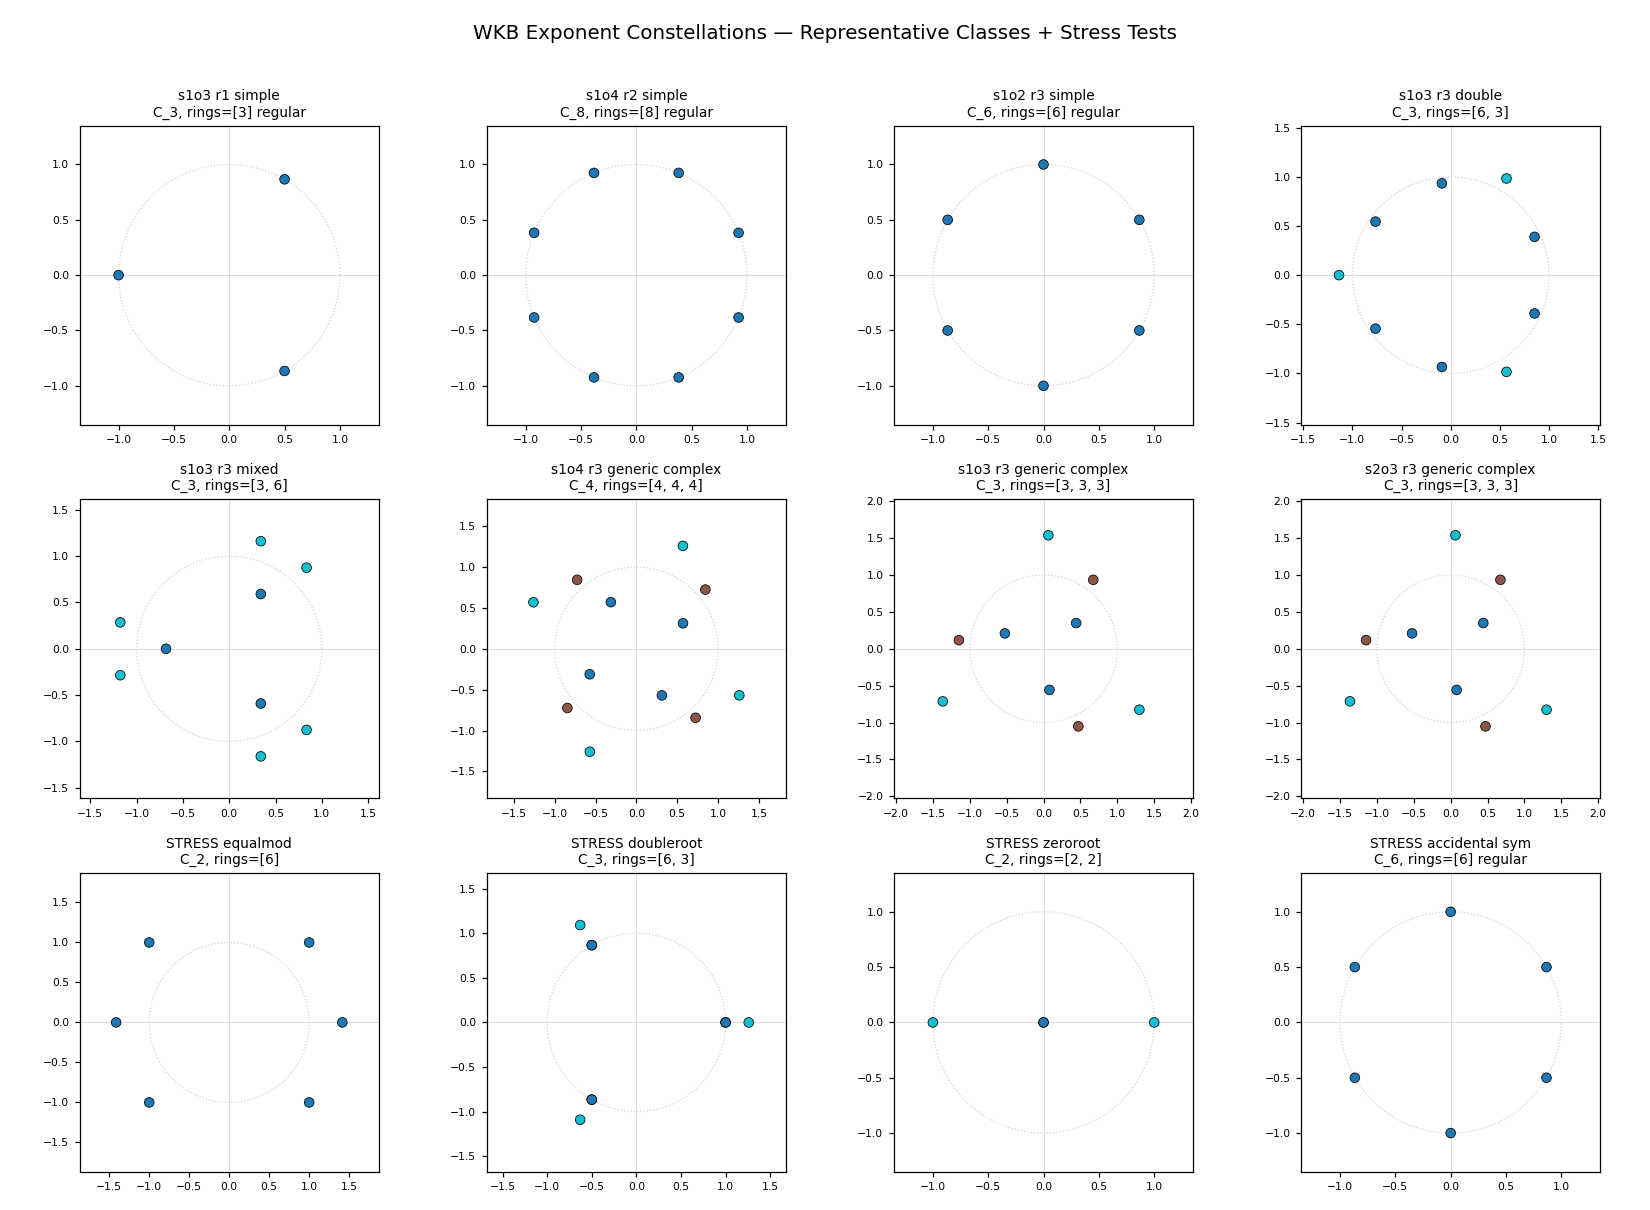
\includegraphics[width=0.95\linewidth]{figures/constellations.png}
\caption{Representative constellations across the $\Fclass$-image. The
$3 \times 4$ grid covers the principal strata. Top row (A1--A4): simple /
binomial classes --- single regular polygon (a single Galois orbit of
$\chi_w$). Middle row (B1--B4): double and generic-complex classes ---
two or three concentric $\mu_q$-orbits. Bottom row (C1--C4): the four
named degenerate strata. Panels A3 and C4 are visually identical $6$-gons
but live in different cells: A3 at slope $1/3$ has minimum symmetry $C_3$
enhanced to $C_6$; C4 at slope $1/2$ has $C_2$ enhanced to $C_6$. The
constellation alone does not recover the cell --- the Newton-polygon
denominator $q$ is required. This is the visible signature that
$\Fclass$ is many-to-one and that accidental symmetry is a feature of
every simple-class operator. The full dataset of plots is in the
companion repository \cite{wkb_dataset_v1}.}
\label{fig:zoo}
\end{figure}

\Cref{fig:zoo} shows twelve representative panels. The full enumeration
of all $23$ classes, with explicit operator representatives, $\chi_w$
data, and panel pointers, lives in the companion dataset
\cite{wkb_dataset_v1}.


%% ============================================================================
%% §9  RELATED WORK
%% ============================================================================
\section{Related work}\label{sec:related}

\paragraph{ADE singularities and discrete classification.}
As a methodological precedent we take the ADE classification of simple
singularities (Arnol'd \cite{arnold1976}, Brieskorn \cite{brieskorn}) and
of finite subgroups of $SU(2)$ (McKay \cite{mckay}): a small discrete
invariant---a Dynkin diagram---organises an apparently heterogeneous zoo
of analytic objects, with strata governed by simple-root combinatorics
and degenerations corresponding to root-system collisions. Our $23$
constellation classes occupy an analogous slot: a finite combinatorial
atlas indexed by the discrete data $(q, r, \pi, \chi_w)$, with degenerate
strata produced by collisions among the inner roots $w_i$ (the analogue
of root coincidences). Unlike the ADE setting, our classes are not
labelled by Dynkin diagrams---the relevant combinatorics is the partition
of $\chi_w$'s roots by modulus and Galois orbit---but the \emph{style} of
classification (discrete invariants, stratified moduli, degeneration
loci) is closely modelled on it.

\paragraph{Formal classification: Levelt--Turrittin and descendants.}
The Levelt--Turrittin theorem (Levelt \cite{levelt}, Turrittin
\cite{turrittin}; modern accounts in Sabbah \cite{sabbah-isomon} and
Sabbah--Mochizuki \cite{mochizuki-asymptotic}) gives a formal
classification of meromorphic connections by \emph{irregular type}: a
multiset of exponential factors $e^{P_i(x^{1/q})}$ together with
regular-singular twists. Birkhoff--Trjitzinsky \cite{birkhoff-trjitzinsky}
and the $q$-difference theories of Sauloy \cite{sauloy}, Ramis
\cite{ramis-stokes,ramis-q-stokes}, and Zhang \cite{zhang} play the
parallel role for difference and $q$-difference operators. Each of these
theories classifies \emph{the operator} up to formal or analytic
equivalence; our object is different. We classify the \emph{image} of
the WKB-extraction functor $\Fclass$, \ie\ the discrete geometry that
$\NL$ and its leading-edge coefficients deposit on the complex plane.
The connection is one-way: the Levelt--Turrittin/Birkhoff--Trjitzinsky
exponents are recovered from $\Cl(L)$ together with auxiliary phase data,
but $\Cl(L)$ itself is coarser and admits a clean independent
classification.

\paragraph{Stokes graphs and spectral networks.}
A third neighbour is the Stokes-graph classification of Painlev{\'e} and
other low-rank equations (Kawai--Takei \cite{kawai-takei},
Iwaki--Nakanishi \cite{iwaki-nakanishi}, Aoki--Kawai--Takei
\cite{aoki-kawai-takei}), and more broadly the spectral-network programme
of Gaiotto--Moore--Neitzke \cite{gmn-spectral}. There, classification
proceeds via the \emph{combinatorial topology of Stokes lines} in the
complex plane, which depends on $c_i - c_j$ rather than $|c_i|$. Our
ring-modulus partition is therefore \emph{not} a Stokes invariant and
does not reproduce spectral-network combinatorics; instead it captures
the strictly weaker but exact information of the multiset $\{c_i^q\}$.
This makes $\Fclass$ a coarsening of the spectral-network functor, which
we view as an asset: the coarser invariant is computable directly from
Newton-polygon data and admits a closed-form classification, whereas
Stokes graphs in general do not.

\paragraph{Wild character varieties and irregular Riemann--Hilbert.}
The geometry of \emph{wild character varieties} and the irregular
Riemann--Hilbert correspondence (Boalch
\cite{boalch-stokes,boalch-wildhodge}, Sabbah \cite{sabbah-polarizable},
Mochizuki \cite{mochizuki-asymptotic}) produces moduli stacks parametrising
local data of irregular connections; our $\Fclass$-image is a discrete
shadow of such a stack restricted to scalar operators with one dominant
edge. We do not attempt to lift the present classification to the level
of stacks or to incorporate Stokes structures intrinsically; rather, we
exhibit a self-contained classification of the discrete part of the local
data, with the analytic refinement of \S\ref{sec:analytic} attaching the
first layer of Stokes information (anti-Stokes directions; slope-graded
Stokes filtration) but stopping short of explicit Stokes constants. The
contribution is best understood as building a separately classifiable
layer of the local picture---a Newton-polygon WKB stratum---on which the
fuller analytic theories can subsequently be erected.


%% ============================================================================
%% §10  DISCUSSION AND VISION
%% ============================================================================
\section{Discussion and future directions}\label{sec:vision}

The natural object of study, in our view, is not any individual operator
but the constellation functor $\Fclass$ itself: the map from
locally-irregular linear models to their WKB exponent multisets. Once
$\Fclass$ is named, the questions become geometric---what is its image,
what are its fibres, what are its strata, how does it deform---and admit
answers in closed form when restricted to one dominant Newton edge. The
$23$ classes catalogued here populate the lowest-dimensional cells of
$\mathrm{Im}(\Fclass)$; their adjacencies trace out the discriminant,
equal-modulus, and zero-root walls along which the structure changes.

The natural sequel is to walk the same programme up the complexity
ladder. \Cref{thm:M1,thm:N1,thm:AT5} already step one rung: multi-edge
Newton polygons (where $\Fclass$ acquires a slope-filtration target) and
nested ramification (where the visible symmetry inflates from $\mu_q$ to
$\mu_{\mathrm{lcm}(q, q')}$). Beyond:
\begin{itemize}[leftmargin=2em]
\item \textbf{Coupled systems.} Matrix and meromorphic-connection systems
      have root systems on each edge; their WKB target is a wild
      character variety. \Cref{thm:S1} treats only the block-diagonal
      case. Genuinely coupled systems (non-semisimple leading symbol)
      lie outside the present classification and connect naturally to
      Boalch's wild non-abelian Hodge theory \cite{boalch-wildhodge}.
\item \textbf{Stokes constants and the analytic refinement.} The
      anti-Stokes skeleton of \Cref{thm:AT1,thm:AT5,thm:AT7} attaches
      \emph{directions} to constellations; the next layer is the
      attachment of \emph{Stokes constants} along each ray. The locus of
      Stokes-equivalent operators above a fixed constellation is the
      kernel of a refined functor $\widetilde\Fclass$ whose image is a
      wild-character-variety stratum.
\item \textbf{Difference and $q$-difference Stokes lifts.} The analytic
      theorems are stated for $\op = \opD$; the analogues for $\opS$
      (Birkhoff--Trjitzinsky) and $\opT$ (Ramis $\theta$-Stokes) require
      separate analytic foundations and are deferred. The constellation
      identities (\Cref{thm:main,thm:M1,thm:N1,thm:D2,thm:S1}) hold
      verbatim across equation types.
\item \textbf{Composite-$q$ Kummer dichotomy.} \Cref{thm:D2} is sharp for
      prime $q$ within the Phase-III search window. The composite-$q$
      version requires the refinement of \Cref{rem:D2-composite} and
      the transcendental-degree statement of \Cref{rem:D2-search}.
\end{itemize}

We expect the functorial reframing to be useful precisely because it
makes a single, universal target geometry visible behind a great many
local stories that, treated one at a time, have looked unrelated. The
classifiable object is the functor; the discrete combinatorics of the
constellation sits transversally to the analytic theory---coarser,
computable, and structurally separable.

%% ============================================================================
%% §11  REPRODUCIBILITY NOTE
%% ============================================================================
\section{Reproducibility note}\label{sec:reproducibility}

All computational artifacts---the operator atlas, characteristic
polynomials, constellations, clusters, conjectures, counterexample
catalogue, taxonomy specification, and rendered figures---are bundled in
the companion Zenodo dataset \cite{wkb_dataset_v1}. The dataset is
organised under the directory structure
\begin{center}
\texttt{/code\ /data\ /figures\ /reports\ /theorems\ /paper-draft\ /fleets}
\end{center}
with \texttt{README.md} at the root. The five fleet pipelines
(\texttt{fleet.py}, \texttt{fleet3.py}, \texttt{fleet4.py},
\texttt{fleet5.py}) are deterministic and self-contained
(\texttt{Python 3.10+}, \texttt{sympy}, \texttt{numpy},
\texttt{matplotlib}); no random seeds are used. Running each fleet in
sequence reproduces the JSON atlas and the rendered constellation zoo
(\texttt{constellations.png}).

The proofs of \Cref{thm:M1,thm:N1,thm:D2,thm:S1,thm:AT1,thm:AT3,thm:AT5,thm:AT7}
are also bundled in the dataset as the file \texttt{proofs.md}, in
long-form expository style with explicit cross-references to
Phase-III/IV evidence. The integration map
(\texttt{integration\_map.md}) records, for each theorem, the dataset
artifact that supplies its empirical evidence. The counterexample
catalogue (\texttt{counterexamples.json}) records the strata on which
naive forms of the theorems fail; each theorem statement above includes
a remark guarding against the relevant counterexamples.

\medskip
\noindent\textbf{Citation.} If you use this work, please cite both the
paper and the dataset; the dataset DOI (placeholder
\texttt{10.5281/zenodo.XXXXXXX}) will be assigned by Zenodo on
publication of v1.0.

%% ============================================================================
%% COMPUTATIONAL AND AI DISCLOSURE
%% ============================================================================
\section*{Computational and AI Disclosure}\label{sec:disclosure}

\paragraph{Computational environment.}
All numerical and symbolic work in this paper was carried out in
\texttt{Python 3.10+} using \texttt{sympy} (exact symbolic algebra),
\texttt{fractions} and \texttt{numpy} (exact rational and floating-point
arithmetic), and \texttt{matplotlib} (figure rendering). No randomised
algorithms were used and no random seeds were set: every JSON artifact
in the companion dataset \cite{wkb_dataset_v1} is reproduced bytewise on
re-execution. The manuscript was typeset with MiKTeX/\TeX{} Live using
the package set listed in the preamble; the bibliography was processed
with \texttt{bibtex} against \texttt{references.bib}.

\paragraph{Automated pipelines (Phases I--V).}
The computational atlas was produced by five fleet scripts, each
implementing one phase of the investigation:
\begin{itemize}[leftmargin=2em,itemsep=2pt,topsep=2pt]
\item \texttt{fleet.py} (Phases I/II) --- generates the single-edge
  operator atlas, computes Newton polygons, extracts characteristic
  polynomials $\chi$ and inner polynomials $\chi_w$, clusters the
  exponent constellations, and emits the initial conjecture list.
\item \texttt{fleet3.py} (Phase III) --- extends the atlas to
  multi-edge polygons, $2\times 2$ and $3\times 3$ systems, resonant
  slopes ($q\le 7$), and nested ramification; computes
  $\Delta_{ij}$ partitions, Galois-orbit invariants, and the
  inner-polynomial $\mathbb{Z}$-resonance dichotomy.
\item \texttt{fleet4.py} (Phase IV) --- lifts the discrete invariants
  to the analytic layer via the Levelt--Turrittin decomposition,
  predicts anti-Stokes rays from the $\Delta_{ij}$ geometry, and
  cross-checks the predictions against numerical Stokes computations.
\item \texttt{fleet5.py} (Phase V) --- consolidates the conjectures
  into theorem--proof pairs, runs each statement against the
  counterexample catalogue, and emits the proof skeletons recorded in
  \texttt{proofs.md} with placements specified by
  \texttt{integration\_map.md}.
\end{itemize}
The pipelines are deterministic and self-contained; running them in
sequence reproduces every JSON file, the rendered constellation zoo
(\texttt{constellations.png}), and the proof skeletons.

\paragraph{Role of AI assistance.}
This work was conducted as independent research with AI-assisted
execution (GitHub Copilot CLI driving an Anthropic Claude Opus~4.7
model). The assistant was used in five clearly demarcated roles:
\begin{enumerate}[label=(\roman*),leftmargin=2em,itemsep=2pt,topsep=2pt]
\item \emph{Conjecture selection.} The assistant scanned the
  Phase-I--III invariant tables for candidate universality laws; the
  author selected which conjectures to promote to the main text.
\item \emph{Proof-skeleton generation.} For each promoted conjecture
  the assistant produced a draft proof skeleton naming the algebraic
  ingredients (Newton-polygon combinatorics, $\mu_q$-pullback,
  $\chi_w$ factorisation, Levelt--Turrittin, determinant polygon);
  the author verified each step and rewrote the load-bearing
  arguments.
\item \emph{Counterexample guarding.} The assistant cross-referenced
  each candidate theorem against \texttt{counterexamples.json} and
  proposed genericity hypotheses (prime $q$, single-edge, non-resonant
  inner polynomial) that survive the catalogued exceptions; the
  author adjudicated which restrictions were accepted into the final
  statements.
\item \emph{Refinement passes.} The assistant unified notation, fixed
  cross-references, and polished prose; all theorem statements,
  remarks, and limitations were reviewed by the author.
\item \emph{Manuscript assembly.} The assistant inserted the
  theorem--proof blocks into the section placements recorded in
  \texttt{integration\_map.md}, assembled the bibliography, and
  produced the arXiv and journal submission bundles.
\end{enumerate}
No proprietary or closed-source models were used beyond the
publicly-available AI assistant named above; no model was fine-tuned on
the project's data, and no AI-mediated literature summaries were used
in place of primary sources for citations.

\paragraph{Human accountability.}
All mathematical statements, theorem formulations, proofs, and
classification claims in this paper were reviewed, validated, and
finalised by the author. In particular, the structural law of
\Cref{thm:main}, the multi-edge and nested-ramification factorisations
of \Cref{thm:M1,thm:N1}, the prime-$q$ Kummer dichotomy of
\Cref{thm:D2}, the system pullback of \Cref{thm:S1}, the four
analytic-lifting theorems \Cref{thm:AT1,thm:AT3,thm:AT5,thm:AT7}, and
the 23-class taxonomy of \Cref{sec:classes} reflect human mathematical
judgment. The author retains sole accountability for all claims,
methodology choices, and the published result.

\paragraph{Reproducibility.}
The complete computational record --- operators, Newton polygons,
characteristic polynomials, constellations, clusters, counterexamples,
Phase-III/IV invariants, proof skeletons, integration map, and
rendered figures --- is deposited as the companion Zenodo dataset
\cite{wkb_dataset_v1}, licensed CC-BY-4.0 (text and data) and MIT
(code and pipelines).
All code, fleet scripts, and sample artifacts are publicly available
at \url{https://github.com/papanokechi/wkb-newton-polygons}, which
mirrors the Zenodo v2.0 dataset and provides a stable, versioned
record of the computational workflow.
The dataset DOI is \texttt{10.5281/zenodo.XXXXXXX}
(placeholder, assigned by Zenodo at publication of v1.0). See
\Cref{sec:reproducibility} for the command sequence that reproduces
every artifact.


%% ============================================================================
%% ACKNOWLEDGEMENTS
%% ============================================================================
\section*{Acknowledgements}\label{sec:ack}

The fleet pipeline that generated the computational atlas was prototyped
in successive phases of automated investigation; the author thanks the
contributors to \texttt{sympy}, \texttt{numpy}, and \texttt{matplotlib},
on which the pipeline rests. Acknowledgements of individual collaborators
and funding sources will be added in the camera-ready version (v2.0).


%% ============================================================================
%% BIBLIOGRAPHY
%% ============================================================================
\bibliographystyle{alpha}
\bibliography{references}

\end{document}
